\chapter{Geometrie auf der Kugeloberfläche\label{chapter:kugel}}
\lhead{Geometrie auf der Kugeloberfläche}
\begin{refsection}
\chapterauthor{Melina Staub und Fabian Schmid}

\section{Einleitung}
Seit jeher fasziniert den Menschen die Fahrt zur See. Nicht grundlos ist die Seefahrt eine der wichtigsten und ältesten Tätigkeiten der Menschheit. Der innerliche Drang neue Weltmeere und unbekannte Gebiete zu entdecken, die Fahrt zur See zu erleichtern und erträglicher zu machen, trieben die Menschen an, die Schiffe dieser Welt immer weiter zu entwickeln.
In der Seefahrt spielte auch die Form der Erde eine wichtige Rolle. Den die Idee der Erde als Kugel ist älter als man zu denken vermag. Bereits der Schüler des antiken griechischen Philosophen Platon - Aristoteles beschrieb in seiner Schrift \textit{Über den Himmel} aus dem 4. Jahrhundert v. Chr. etliche Gründe welche für die Gestallt der Erde als Kugel sprechen:
\begin{itemize}
      \item Sämtliche schweren Körper streben zum Mittelpunkt des Alls. Da sie dies von allen Seiten her gleichmässig tun und die Erde im Mittelpunkt des Alls steht, muss sie eine kugelrunde Gestalt annehmen. 
\item Bei von der Küste wegfahrende Schiffen wird der Rumpf vor den Segeln der Sicht verborgen. 
\item In südlichen Ländern erscheinen südliche Sternbilder höher über dem Horizont.
\item Der Erdschatten bei einer Mondfinsternis ist stets rund.
\end{itemize}

Jedoch war um 1492 - der Zeit der Entdeckung Amerikas durch Christoph Kolumbus, die Idee der Erde in Kugelform noch sehr umstritten. Er erkannte anhand Theorien und Erkenntnissen der alten Griechen, vor jenen von Aristoteles, das die Erde eine Kugel sein muss. \\
Mit seinem Vorschlag einen Seeweg über den Atlantik nach Indien zu finden und nicht wie üblich um Afrika zu segeln, stiess er beim beim portugiesischen König auf taube Ohren. Sein Plan Indien über eine Route nach Westen zu erreichen, widersprach dem gesunden Menschenverstand. Wäre die Erde wirklich eine Kugel und man befände sich auf der unteren Erdhalbkugel, würde man dann nicht herunterfallen? Jedoch brachte auch der damals übliche Glaube an die Erde in Scheibenform brachte so einige Risiken mit sich. Was würde passieren, wenn die Flotte das Ende der Scheibe erreicht hatte? Würden sie über den Erdrand hinweggleiten und in den Abgrund stürzen?\\
Erst nach viel Überzeugungsarbeit durch Kolumbus, setzte er sich am Spanischen Hof durch und segelte über die Westliche Route über den Atlantik und entdeckte schlussendlich Amerika - nicht Indien.
Der praktische und greifbare Beweis das die Erde eine Kugel ist, lieferte rund 30 Jahre später der Portugiese Fernando Magellan. Mit seiner Weltumsegelung und der Ankunft in den Philippinen, bewies er definitiv das die Erde eine Kugel ist.\\

Nun wollen wir uns die Frage stellen, wie die alten Seefahrer ohne GPS und jeglichen modernen Navigationssystemen auf hoher See wussten wo sie sich befanden und was die Sterne mit alledem zu tun haben. Reisen Sie mit uns zurück in eine Zeit der Sextanten, Kompasse und Sternkarten. In die Zeit der Seefahrer und Entdecker.



\section{Gross- und Kleinkreise}
Eine Kugeloberfläche lässt sich in zwei verschiedene Kreisarten einteilen  Gross- und Kleinkreise. 
Wir betrachten als erstes die Grosskreise:


\subsection{Grosskreise}
Es gibt unendlich viele Möglichkeiten eine Kugel in zwei gleich grosse Stücke zu zerschneiden, daher gibt es auch unendlich viele Grosskreise.

\begin{definition}
\textit{Ein Grosskreis ist ein grösstmöglicher Kreis auf einer Kugeloberfläche. Sein Mittelpunkt fällt immer mit dem Mittelpunkt der Kugel zusammen und ein Schnitt auf dem Grosskreis teilt die Kugel auf jedem Fall in zwei (gleich grosse) Hälften.}
\label{skript:kugel:satz:Grosskreis}
\index{Grosskreis}
\end{definition}

\begin{center}
        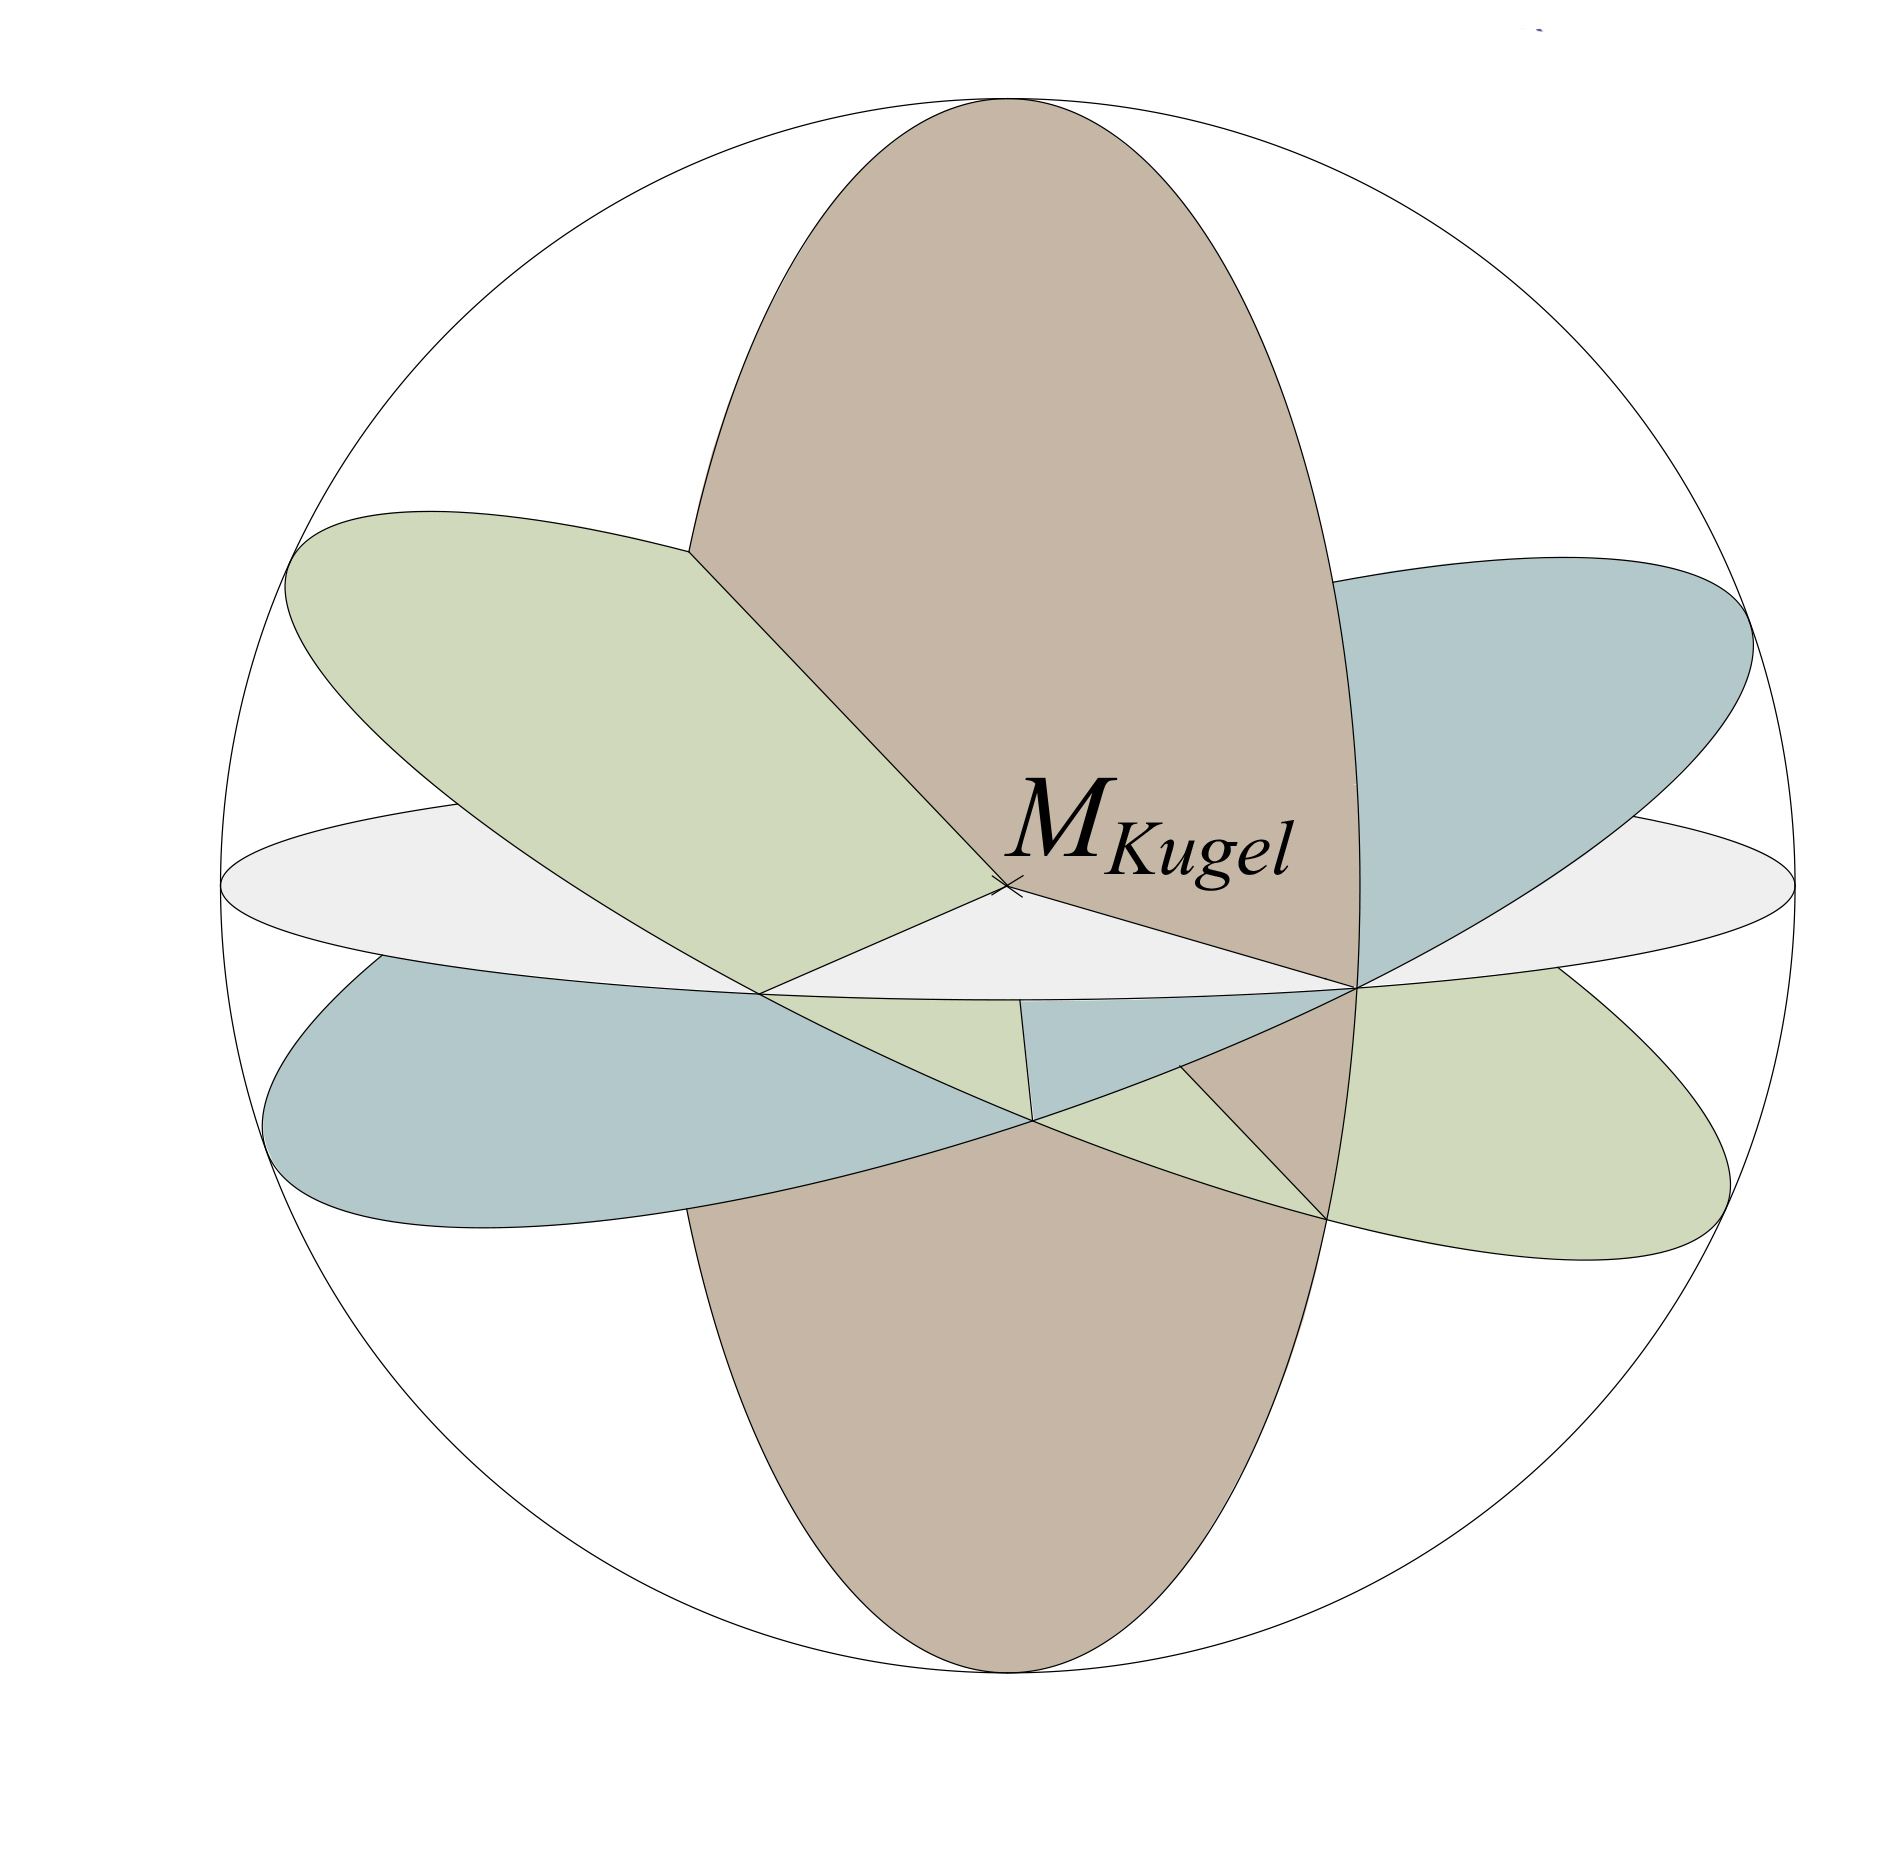
\includegraphics[width=0.4\textwidth]{kugel/_Grosskreis.jpg}
    \captionof{figure}{Verschiedene Grosskreise in einer Kugel}
\end{center}

Ein Elementarer Bestandteil bilden die Grosskreise in der sphärischen Trigonometrie. Mithilfe der Schnittpunkte verschiedener Grosskreise, lassen sich sphärische Dreiecke bilden auf welchen sich die sphärische Trigonometrie anwenden lässt. \\

Um unseren Standort auf der Erde klar zu bestimmen, wurde diese in ein Raster von Grosskreisen unterteilt. Diese stehen orthogonal zum Äquator und sind uns bekannt als Längengrade.


\subsection{Kleinkreise}
Die Kleinkreise eignen sich im Gegensatz zu den Grosskreisen \textit{nicht} für die sphärische Trigonometrie.  Dies liegt daran, dass sie keinen einheitlichen Mittelpunkt haben und so je nach Radius verschieden gross sind.
Sie werden lediglich zur Bestimmung der Messgrössen, Winkelabstände oder des Höhenwinkels eines Gestirns verwendet. 

\begin{definition}
Unter Kleinkreis versteht man jene Kreise auf einer Kugeloberfläche, deren Ebenen nicht den Kugelmittelpunkt enthalten, davon ausgenommen ist der Äquator.
\label{skript:kugel:satz:Kleinkreis}
\index{Kleinkreis}
\end{definition} 

\begin{center}
        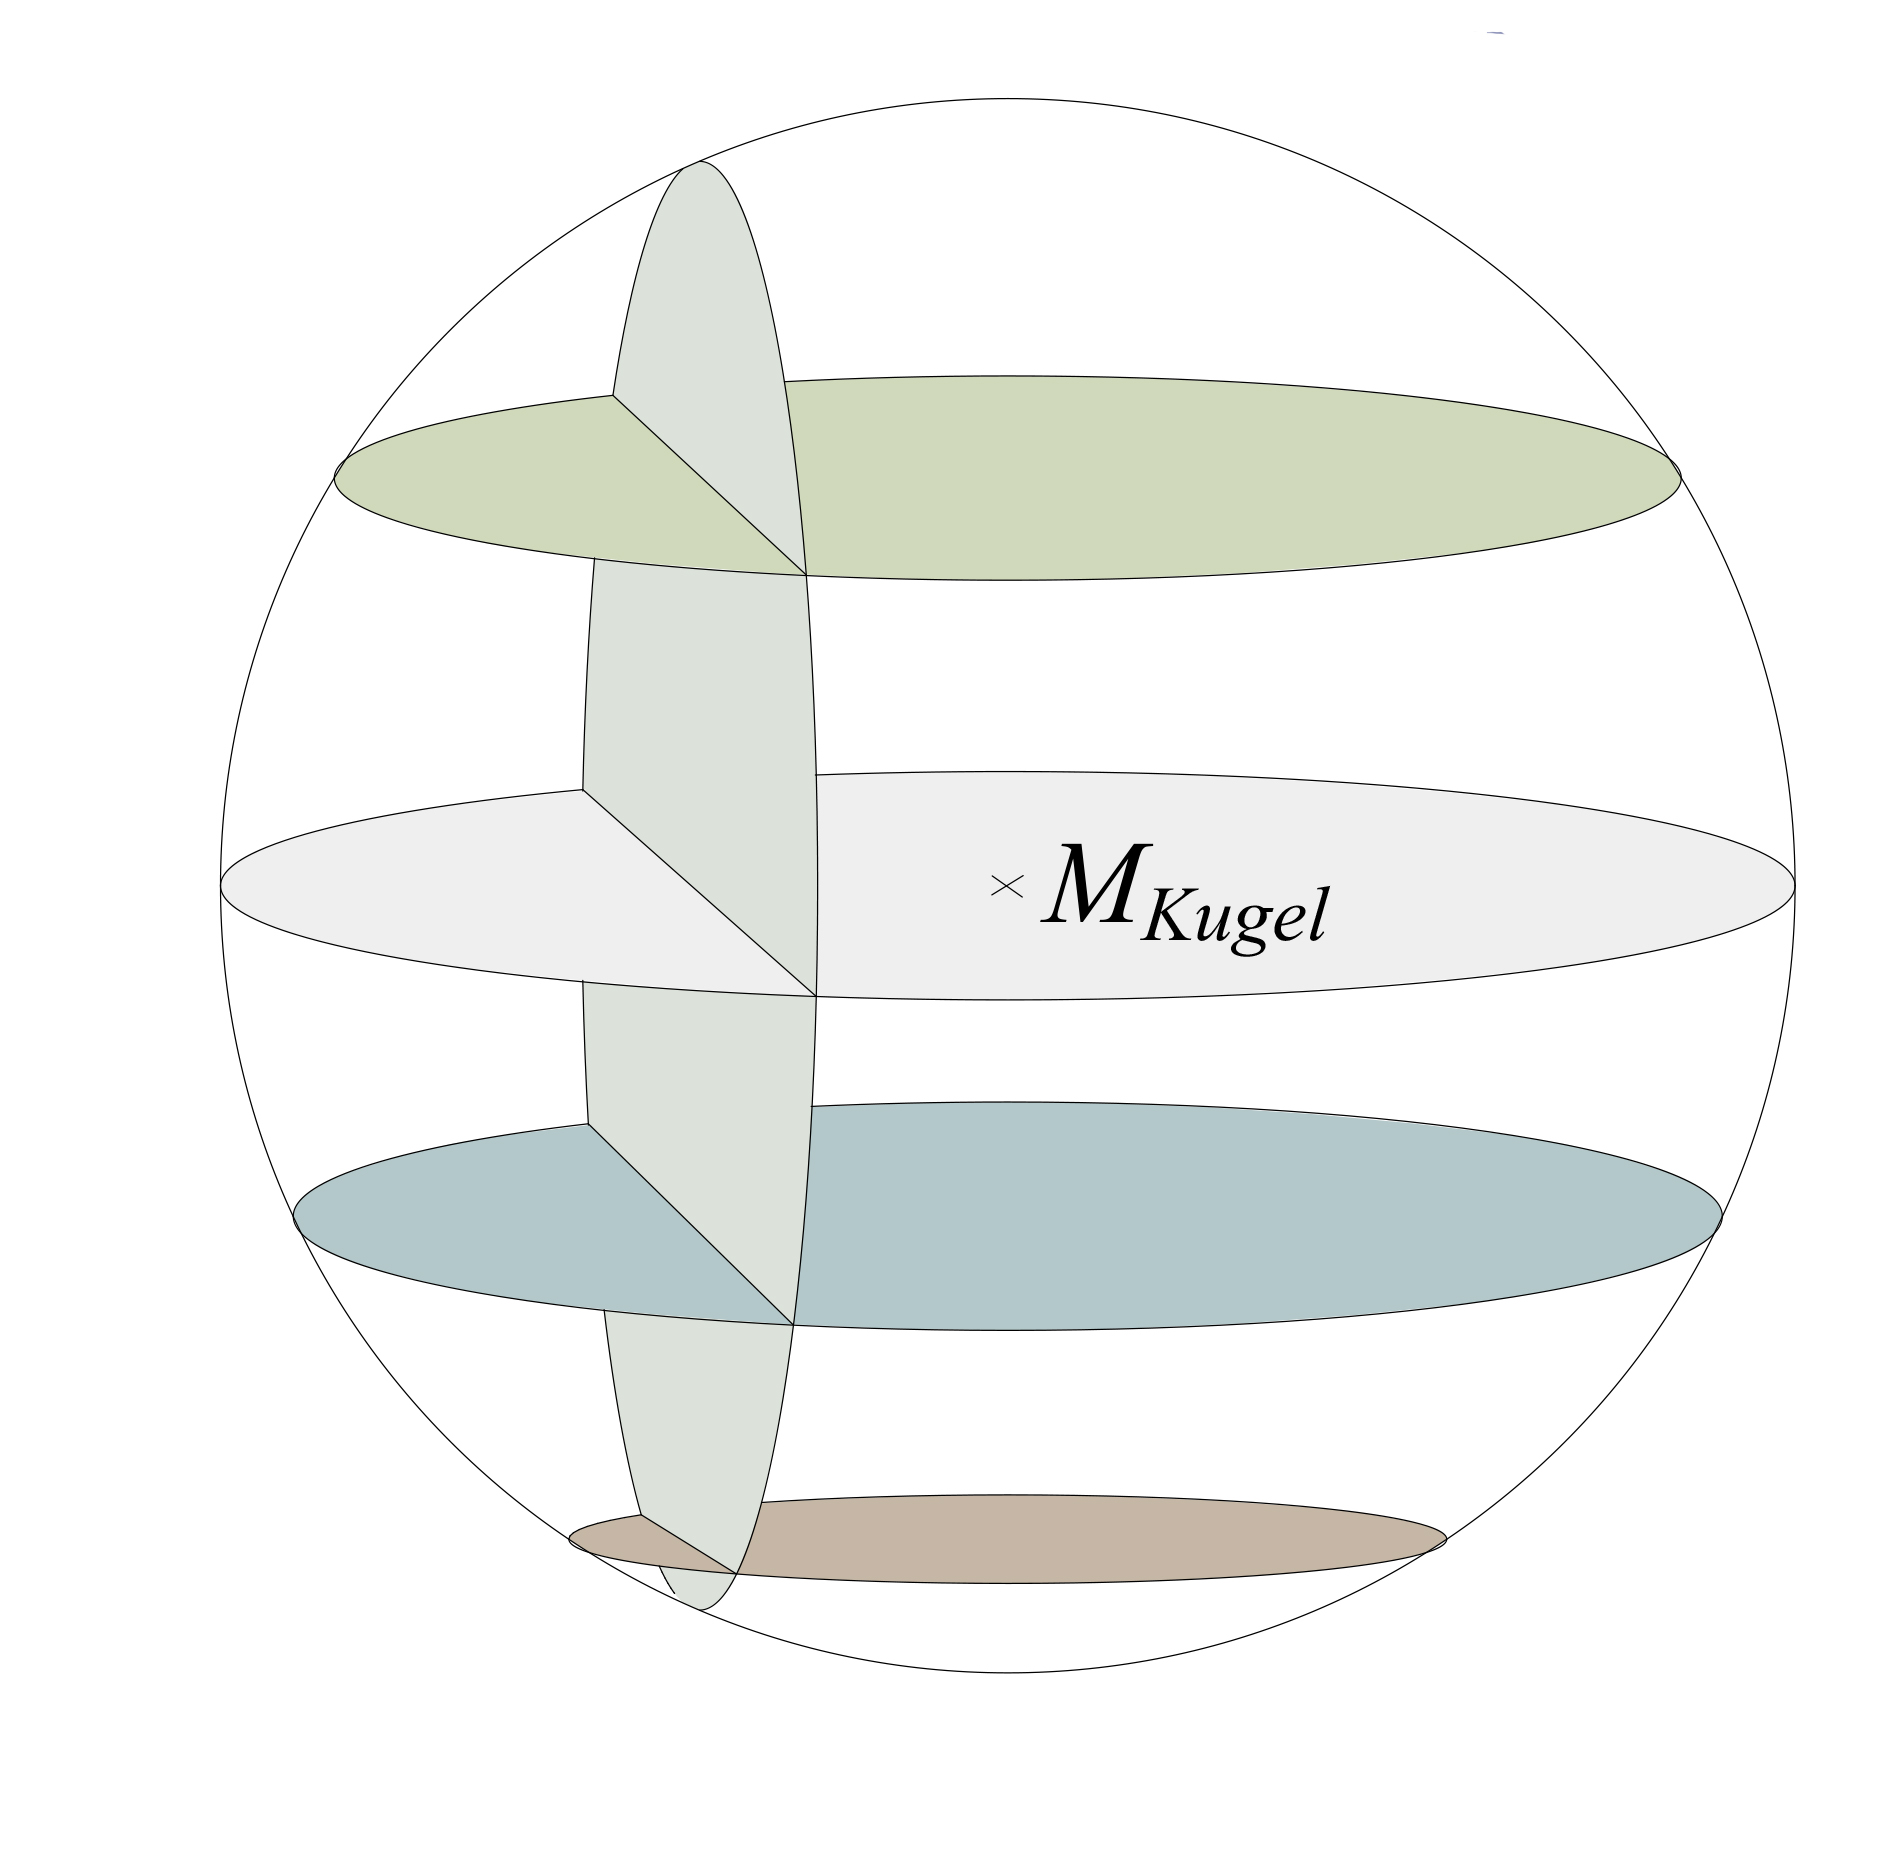
\includegraphics[width=0.4\textwidth]{kugel/_Kleinkreis.jpg}
    \captionof{figure}{Verschiedene Kleinkreise in einer Kugel}
\end{center}

Um unser Raster auf der Erdoberfläche zu vervollständigen und einen klaren Ort auf dem Längengrad zu definieren benutzen wir die Kleinkreise. Diese verlaufen parallel zum Äquator in Richtung Nord und Süd. Der Äquator beschreibt einen speziellen Kleinkreis, da er einen grösstmöglichen Kreis auf der Kugel bildet und somit auch ein Grosskreis darstellt.//
Für die Navigation sind sowohl die für die sphärische Trigonometrie hilfreichen Grosskreise (Längengrade) von Nöten wie auch die Kleinkreise (Breitengrade), da man nur mit beiden in Kombination seine Koordinaten eindeutig bestimmen kann.



\section{Sphärische Dreiecke / Kugeldreieck}
Der Begriff sphärisches Dreieck oder Kugeldreieck ist ein sehr weitläufiger Begriff und wird folgendermassen definiert

\begin{definition}
Ein sphärisches Dreieck oder Kugeldreieck genannt ist eine durch drei Grosskreise begrenzte Figur auf der Kugeloberfläche.
\end{definition} 

Dabei können wir sphärische Dreiecke in drei für uns wesentliche Dreiecksarten unterteilen:

\begin{itemize}
\item Allgemeine Kugeldreiecke (Nicht Eulersche’ Dreiecke)
\item Kugelzweiecke
\item Eulersche’Dreiecke
\end{itemize}


\subsection{Allgemeine Kugeldreiecke (Nicht Eulersche’ Dreiecke)}
Ähnlich dem Dreieck in der Ebene hat das Dreieck auf der Kugel Seiten und Winkel. Allerdings werden die Dreiecksseiten nicht in der Längenmass Meter angegeben sondern im Bogenmass. Den es handelt sich um Kreisbögen und keine Strecken.
Allerdings ist die Winkelsumme eines Kugeldreiecks immer grösser als $180^{\circ}$ und kann bis zu $900^{\circ}$ anwachsen.

\begin{center}
        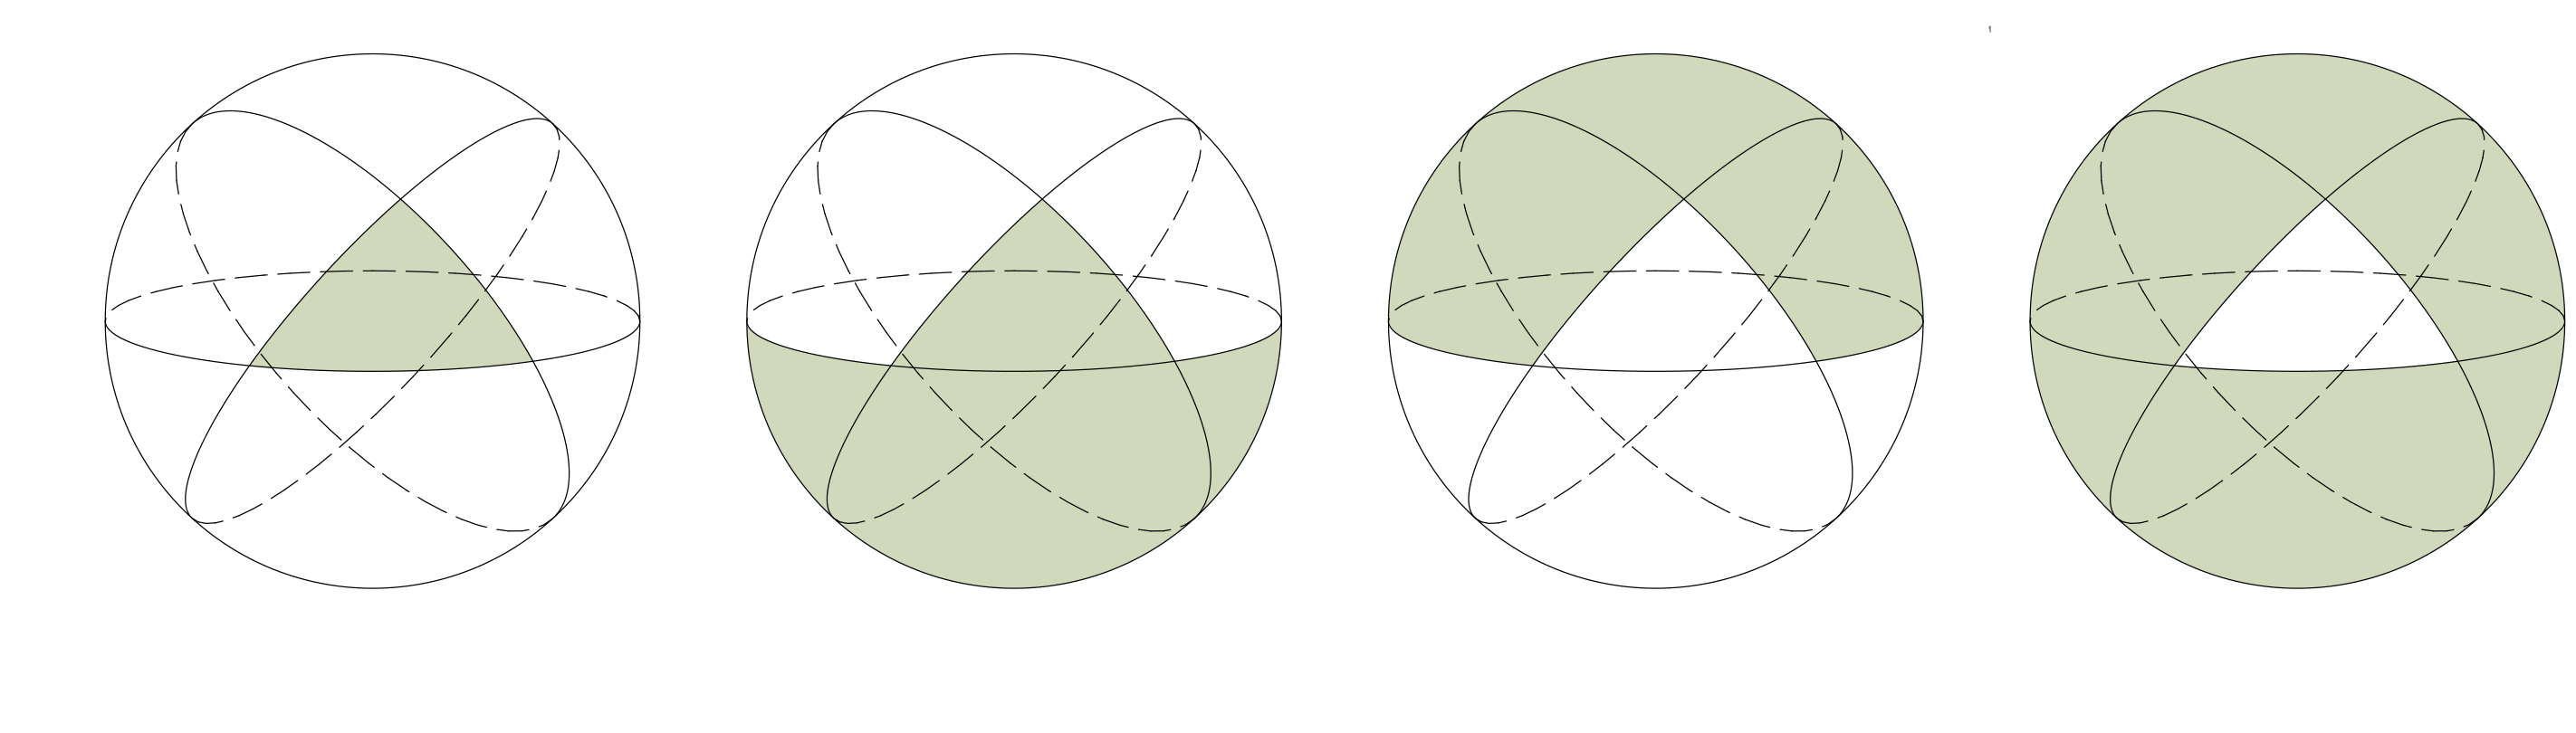
\includegraphics[width=0.9\textwidth]{kugel/_Dreiecksarten.jpg}
    \captionof{figure}{Verschiedene Kugeldreiecke}
\end{center}


\subsection{Kugelzweiecke} 
Zwei Grosskreise auf der Kugeloberfläche zerlegen diese in vier gleich grosse Kugelzweiecke, welche je einen Viertel der Kugeloberfläche abdecken. 
Jedes dieser entstandenen Dreieckseiten hat die Länge
$180^{\circ}$ oder $\pi$.
Der Flächeninhalt wird dabei einzig durch den Winkel $\alpha$ zwischen den beiden Grosskreisen bestimmt.

\begin{center}
        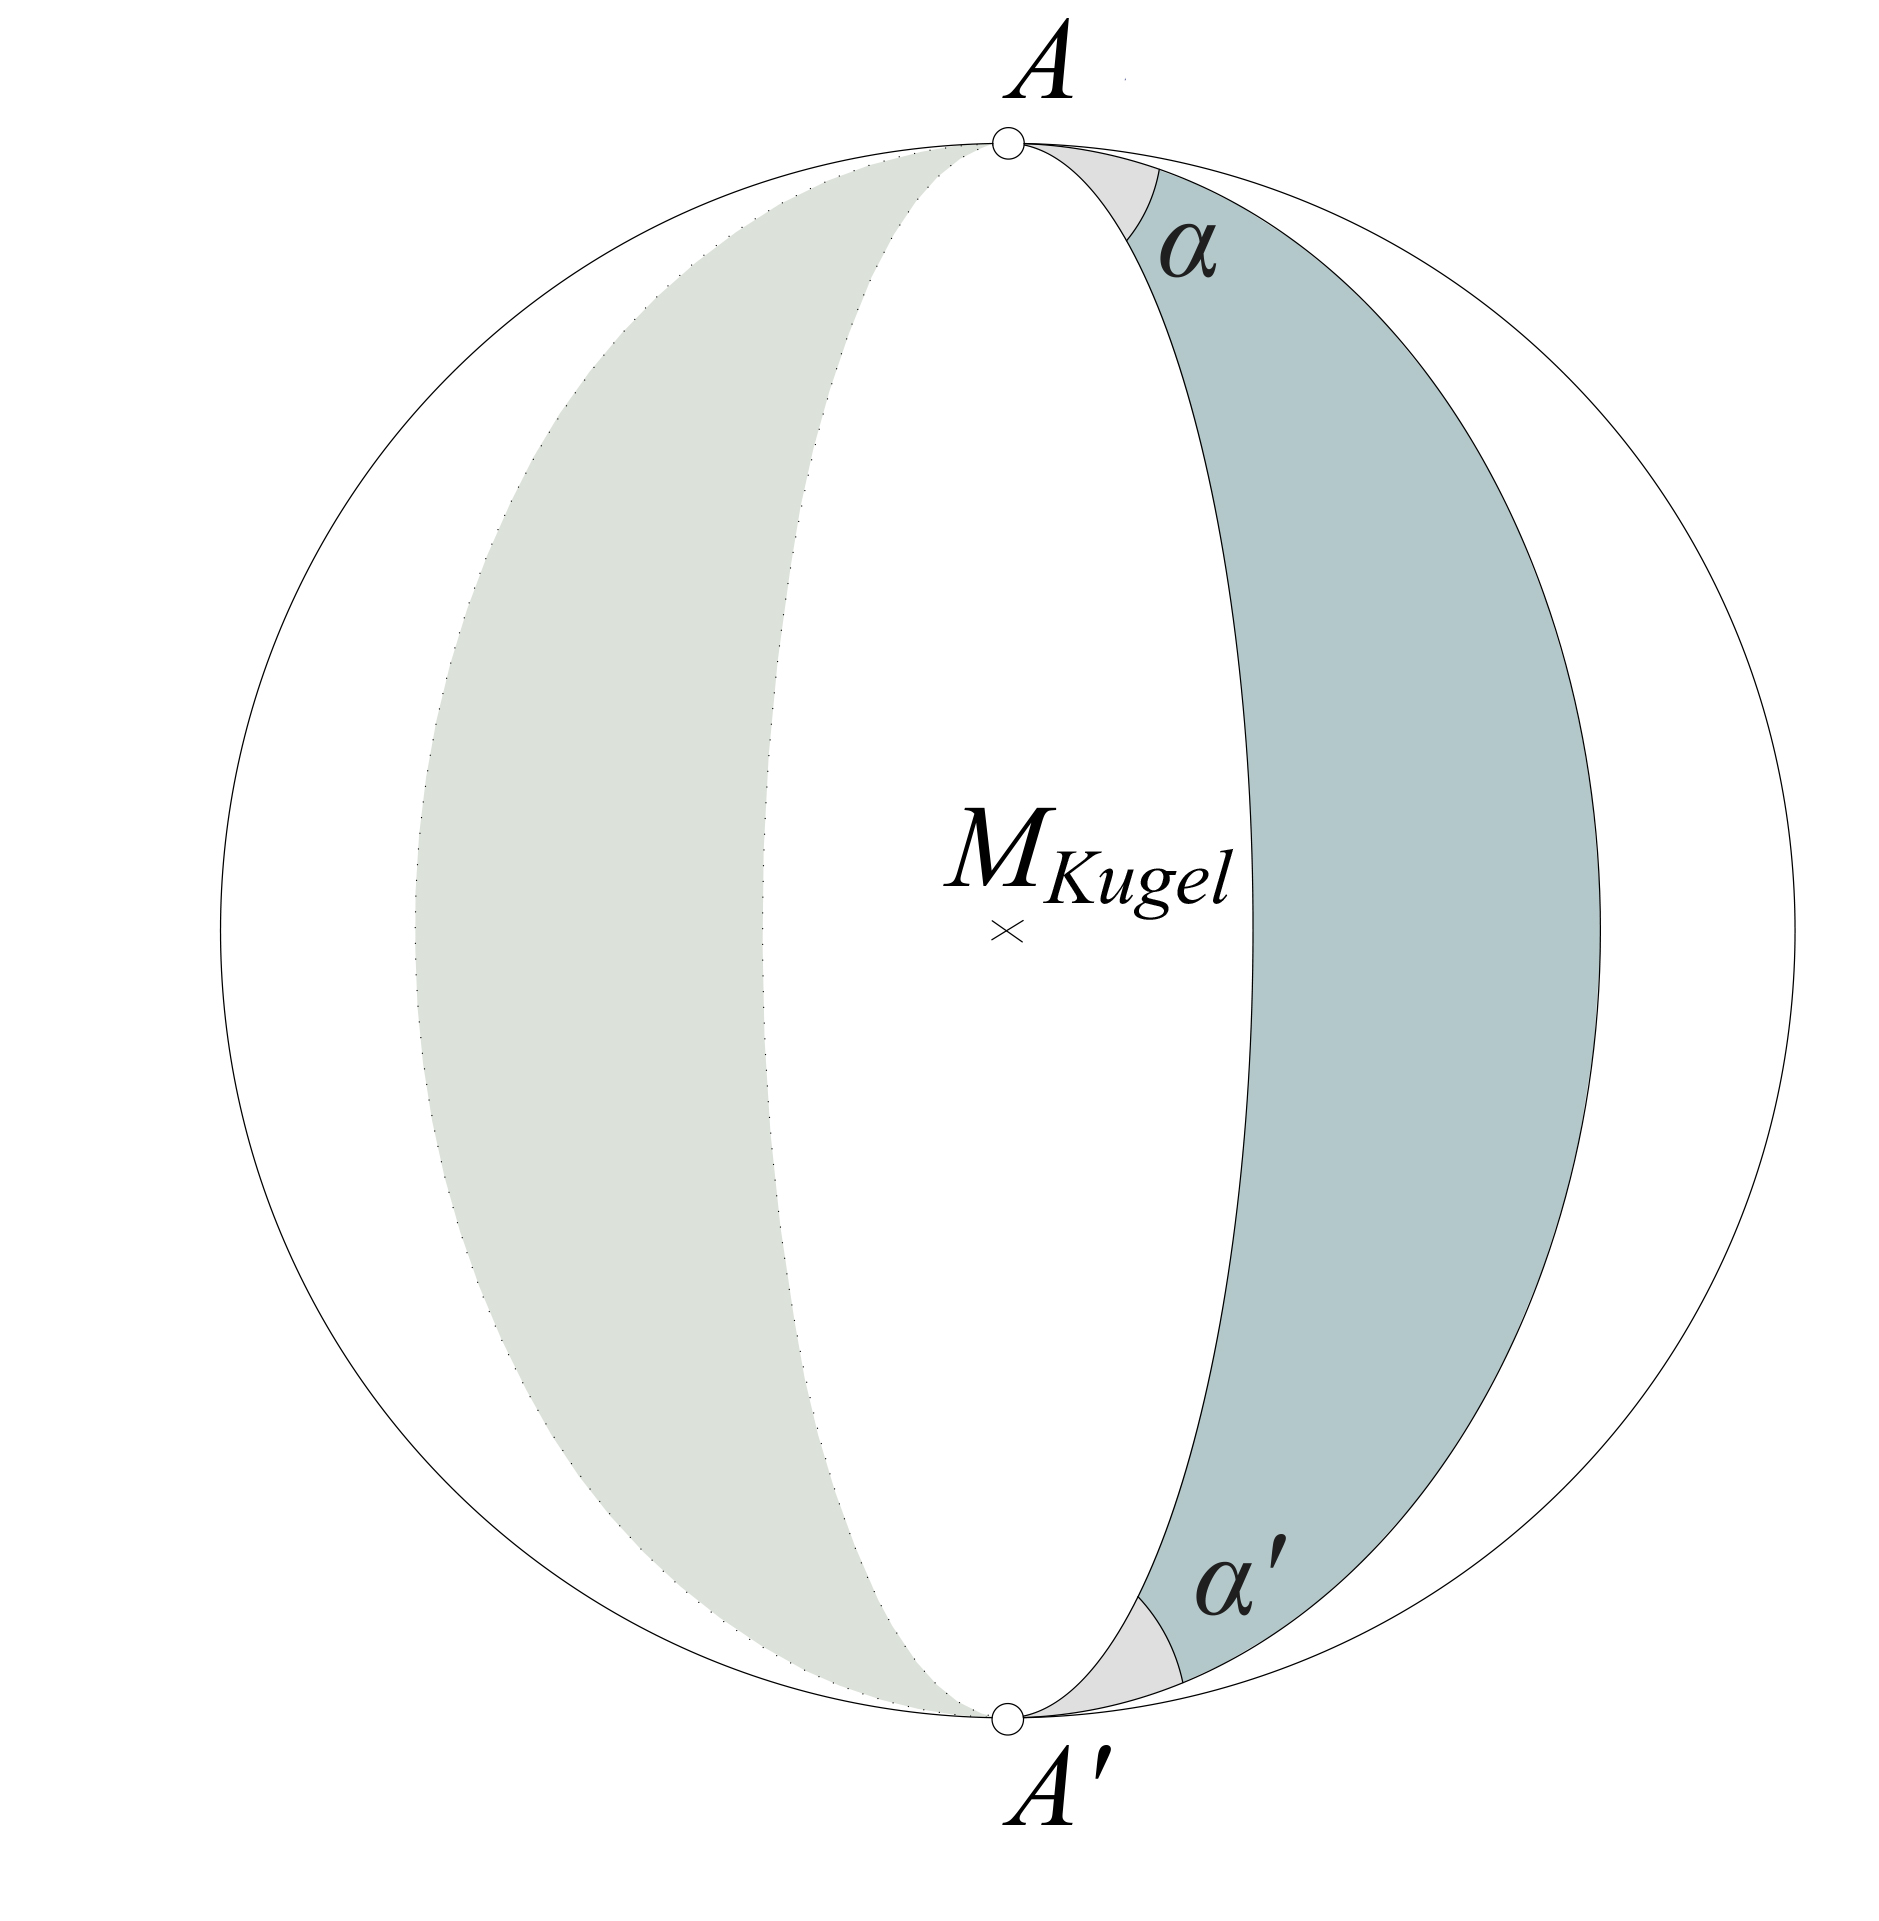
\includegraphics[width=0.4\textwidth]{kugel/_Zweieck.jpg}
    \captionof{figure}{Bildung von Zweiecken durch Grosskreise}
\end{center}

Dabei deckt der Flächeninhalt des Zweiecks einen Teil der Kugeloberfläche ab, sprich

XXXX

Der Flächeninhalt des Zweiecks beschreibt sich unteranderen mit dem Flächeninhalt der Kugel
\begin{align*}
A_{ Kugel } &= 4 \pi r^{2}
\end{align*}

Um den Flächeninhalt des Zweiecks zu erhalten, multiplizieren wir den Flächeninhalt der Kugel $A_{ Kugel }$ mit dem des Kugelsegments des Winkels $\alpha$ 
\begin{equation}
A_{ Zweieck } = 4 \pi r^{2} \cdot \frac{ \alpha }{ 2 \pi } = 2 \alpha r^{2}
\end{equation}

Auf der Erdoberfläche finden wir Vierundzwanzig uns allbekannte Zweiecke - Die Zeitzonen. Auf dieses Thema gehen wir im Kapitel~\ref{Zeitzonen} \nameref{Zeitzonen} näher ein.


\subsection{Eulersche’ Dreiecke} \label{Euler} 
Legt man drei Grosskreise auf eine Kugeloberfläche, bilden sich dabei acht Dreiecke. 
Ein solches Dreieck heisst Eulersches’Dreieck\footnote{%
Leonard Euler (1707-1783), berühmter Schweizer Mathematiker und Physiker. 
Nicht Eulersche’Dreiecke erhält man, indem man das Äussere des Dreieckes ABC betrachtet.}.
Diese werden weder durch die Verlängerung ihrer Seiten durchschnitten, 
noch haben sie Dreiecksseiten welche grösser sind als $180^{\circ}$.

\begin{center}
        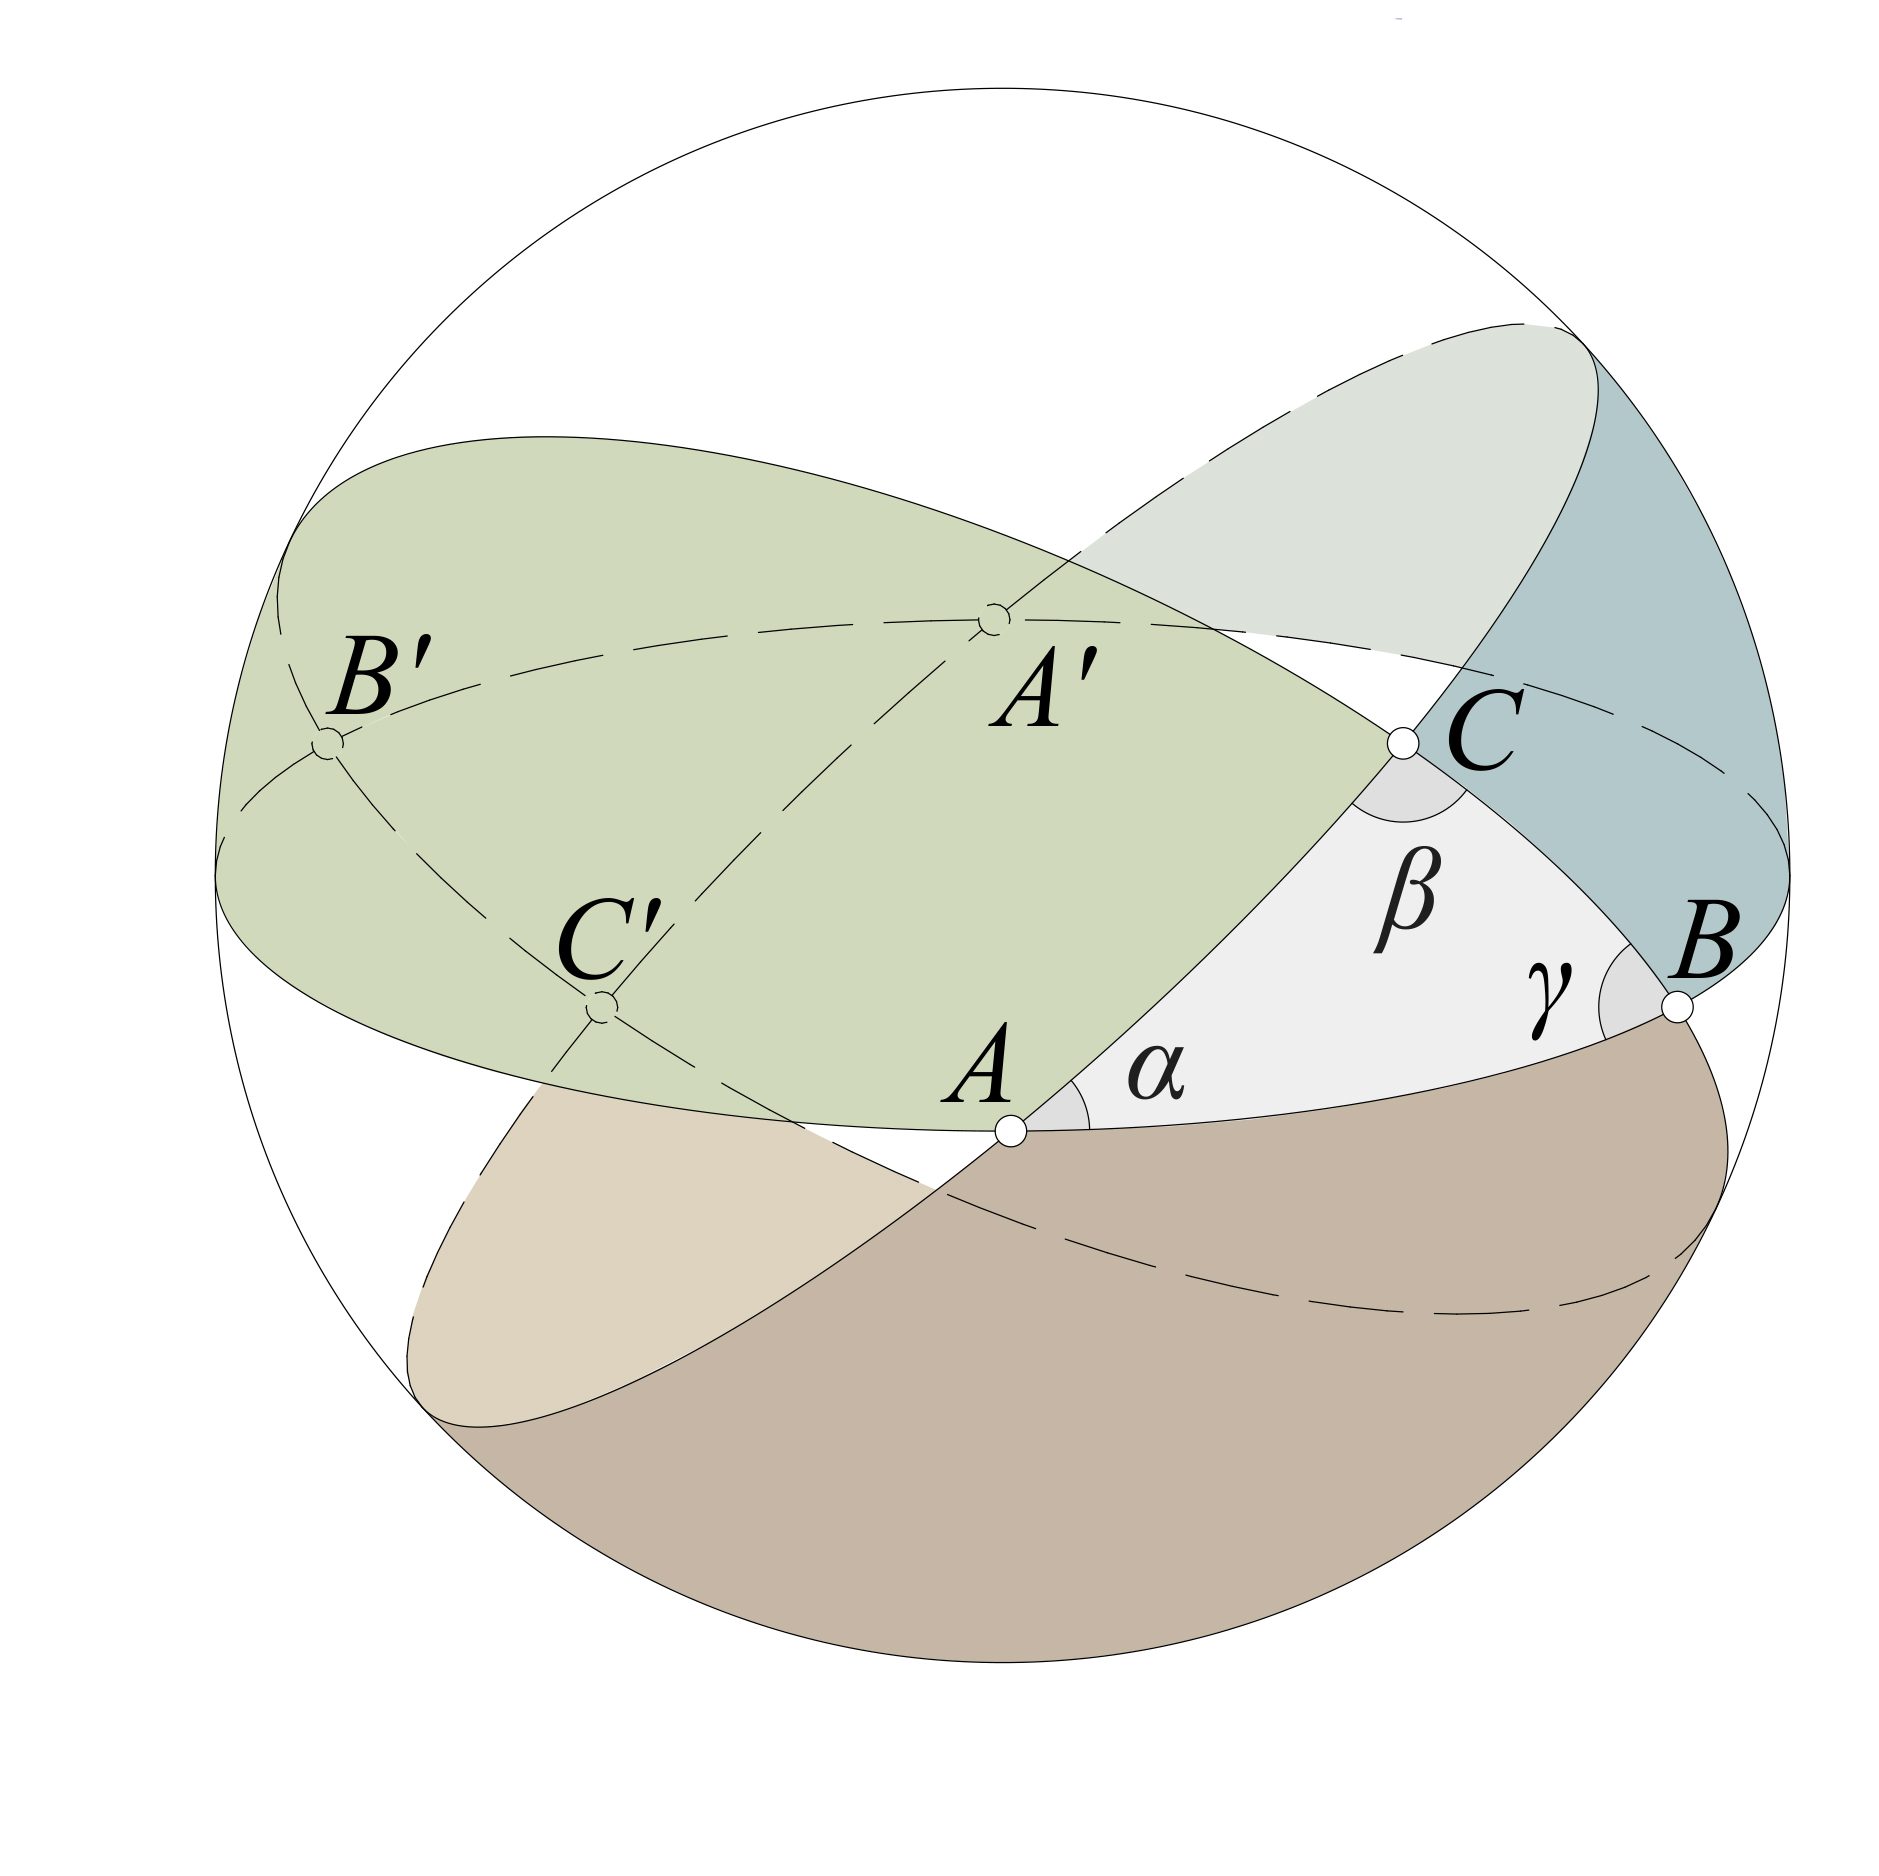
\includegraphics[width=0.4\textwidth]{kugel/_Eulersches.jpg}
    \captionof{figure}{Drei Grosskreise bilden acht Eulersche Dreiecke}
\end{center}

In den nachstehenden Erklärungen und Herleitungen, sprechen wir ausschliesslich von Eulerschen Dreiecken, da die umgeformten Winkelsätze der ebenen Trigonometrie nur auf diese Art von Kugeldreiecken angewendet werden können.

Aus der Ebenen Trigonometrie folgt die Formel für die Innenwinkelsumme aus dem Wechselwinkelsatz
\begin{align*}
\alpha + \beta + \gamma &= 180^{\circ}
\end{align*}

Für die Innenwinkelsumme in der sphärischen Trigonometrie gilt dies nicht. Obschon die Trigonometrie der Sphäre einige Gemeinsamkeiten zu dieser der Ebene aufweist, kann nicht alles übernommen werden.
So auch nicht wie Innenwinkelsumme in einem Eulerschen Dreieck.
Denn diese liegt zwischen
\[
\begin{aligned}
\pi
&\text{ bis }
3\pi
&
&\text{oder}
&
180^{\circ}
&\text{ bis }
540^{\circ}
\end{aligned}
\]
Daraus können wir schliessen, das ein einzelner Winkel durchaus die Grösse $180^{\circ}$ oder $\pi$ annehmen kann, jedoch nicht mehr. Ansonsten wäre es ein allgemeines Kugeldreieck und kein Eulersche’s. Dies würde wiederum bedeuten, dass wir die sphärische Trigonometrie nicht anwenden dürften.



\section{Dreiecksfläche und sphärischer Exzess} \label{Flaeche} 
Betrachten wir das hellgraue Dreieck in der Abbildung 13.5 ist $A_{ \triangle{ ABC }}$ und dessen Flächeninhalt. Der Flächeninhalt $A_{ \triangle{ ABC }}$ berechnet sich aus den Winkeln $\alpha$, $\beta$, $\gamma$ und dem Kugelradius $r$ im Quadrat.
\begin{align*}
A_{ \triangle{ ABC }} &= (\alpha + \beta + \gamma - \pi) \cdot r^2
\end{align*}

Das diese Formel wirklich zum gewünschten Flächeninhalt führt, lässt sich folgendermassen beweisen:\\
Als erstes berechnen wir die einzelnen Flächeninhalte der Zweiecke A, B und C
\begin{align*}
\text{Zweieck A}
&=
\triangle{ABC} + \triangle{A'BC} = 2 \alpha r^{ 2 } = A_{ \alpha }\\
\text{Zweieck B}
&=
\triangle{ABC} + \triangle{AB'C} = 2 \beta r^{ 2 } = A_{ \beta }\\
\text{Zweieck C}
&=
\triangle{ABC} + \triangle{ABC’} = 2 \gamma r^{ 2 } = A_{ \gamma }
\end{align*}

Die drei Zweiecke und zweimal das kleine graue Eulersche’ Dreieck bedecken zusammen  die halbe Kugel was in der Abbildung 13.6 ersichtlich ist.

\begin{center}
        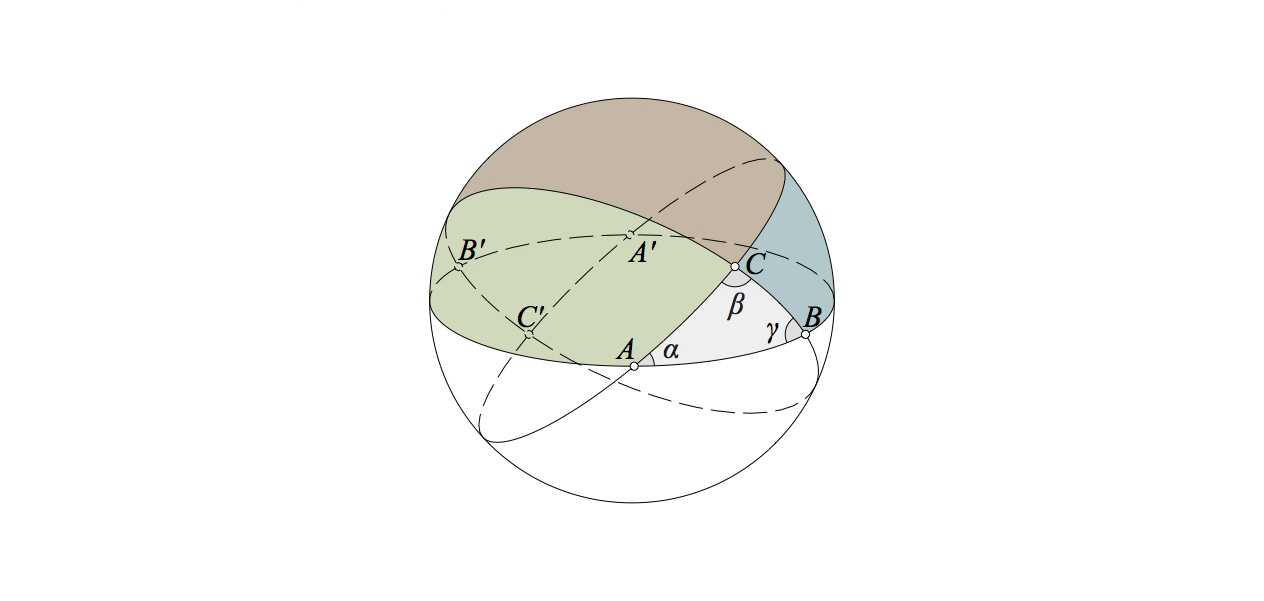
\includegraphics[width=0.4\textwidth]{kugel/1HalbeKugel.jpg}
    \captionof{figure}{Bild FLäche dreieck}
\end{center}

Nun setzen wir die Flächeninhalte der Zweiecke mit dieser der halben Kugel gleich
\begin{align*}
A_{ \alpha } + A_{ \beta } + A_{ \gamma } &= \frac{ 4\pi r^{ 2 } }{ 2 } + 2A_{ \triangle{ ABC }}
\end{align*}

Durch die Division mit Zwei und das Subtrahieren von $\pi r^2$ schreiben wir die Formel des Flächeninhaltes und haben somit folgenden Satz bewiesen
\begin{satz} \textit{Der Flächeninhalt eines Eulerschen Dreiecks verhaltet sich wie die Summe dessen Winkel subtrahiert mit $\pi$ und dessen Differenz multipliziert mit dem Radius im Quadrat.}
\label{skript:kugel:satz:Flaecheninhalt}
\index{Flaecheninhalt}
\end{satz}

\begin{align*}
r^{ 2 }\underbrace{(\alpha + \beta + \gamma - \pi)}_{\text{Sphärischer Exzess}} &= A_{ \triangle{ ABC }}  
\end{align*}

Dabei beschreibt die Winkelsumme abzüglich $\pi$ den sphärischen Exzess im Kugeldreieck.
Der sphärische Exzess $\epsilon$ gibt dabei an, wie stark die Innenwinkelsumme von $\pi$ abweicht und wird gleichmässig auf alle Winkel verteilt. Dies hat mit der gekrümmten Oberfläche der Kugel zu tun.
\begin{equation}
\epsilon = \alpha + \beta + \gamma - \pi
\end{equation}

\begin{center}
        \includegraphics[width=0.3\textwidth]{kugel/Beispielbild.jpg}
    \captionof{figure}{Bild Sphärischer Exzess}
\end{center}

Folglich ist der Exzess direkt mit dem Flächeninhalt $\triangle A$ eines Eulerschen Dreiecks verbunden
\begin{align*}
\epsilon =\frac{A_{\triangle{ ABC }}}{r^2} = \frac{\alpha + \beta + \gamma - \pi}{r^2}
\end{align*}

Ist der sphärische Exzess und der Flächeninhalt bekannt, kann man mit dessen Hilfe auf einem beliebigen Eulerschen Dreieck auf dessen Radius schliessen.
\begin{align*}
r = \sqrt{\frac{\alpha + \beta + \gamma - \pi}{\epsilon}}
\end{align*}

Mit einer maximalen Innenwinkelsumme bei Eulerschen Dreiecken von $540^{\circ}$ ist der Exzess im Einheitskreis maximal $360^{\circ}$.
\[
\begin{aligned}
180^{\circ} \le \epsilon \le 360^{\circ}
&
&\text{oder}
&
&\pi \le \epsilon \le 2\pi
\end{aligned}
\]

Berechnen wir den maximalen sphärischen Exzess bei allgemeinen Kugeldreiecken würde dieser maximal $720^{\circ}$ annehmen.
\[
\begin{aligned}
180^{\circ} \le \epsilon \le 720^{\circ}
&
&\text{oder}
&
&\pi \le \epsilon \le 4\pi
\end{aligned}
\]



\subsection{Grenzfall - Satz von Legendre}
Würden wir den sphärischen Exzess in der ebenen Trigonometrie anwenden, wäre dieser $=0$. Betrachten wir nun sehr kleine Kugeldreiecke oder solche mit grossen aber endlichen Radien, im Vergleich zur gesamten Kugeloberfläche, würde die Innenwinkelsumme $\pi$ nur wenig übersteigen. Dies besagt, das wir sphärische Dreiecke mit geringer Grösse durch Verebnung annähernd als solche der ebenen Trigonometrie betrachten können. Diese Erkentnis beschreibt der Satz von Legendre

\begin{center}
        \includegraphics[width=0.3\textwidth]{kugel/Beispielbild.jpg}
    \captionof{figure}{Bild Krümmung Gross und Klein}
\end{center}

\begin{quote} \textit{Ein kleines sphärisches Dreieck kann näherungsweise 
wie ein ebenes Dreieck mit denselben Seiten berechnet 
werden, wenn alle Winkel des ebenen Dreiecks die um 
je ein Drittel des sphärischen Exzesses verminderten 
Winkel des sphärischen Dreiecks nimmt.} \end{quote}
\begin{flushright} - Adrien-Marie Legendre (1752-1833), Paris 1787
\end{flushright}

Durch diesen Satz lässt sich der Zusammenhang zwischen der Ebenen Trigonometrie und dieser auf der Kugel herstellen.



\section{Sphärisch Analoge Winkelfunktionen}
Euklid von Alexandria\footnote{%
Euklid war ein griechischer Mathematiker. Er lebte wahrscheinlich 3 Jahrhunderte vor Christus. In seinem berühmtesten Werk \textit{Euklids Elemente} fasst er die Arithmetik und Geometrie seiner Zeit zusammen. \textit{Euklids Elemente} war 2000 Jahre lang als Lehrbuch in gebrauch und war bis Mitte des 19. Jahrhunderts nach der Bibel das weit verbreitetste Buch der Weltliteratur.}  beschrieb die Grundbegriffe der ebenen Geometrie mittels Punkt, Geraden, Ebene, Winkel und Dreieck. Ebendiese Dreiecke lassen sich mithilfe der ebenen Trigonometrie beschreiben. Dabei gelten die uns bekannten trigonometrischen Winkelfunktionen:\\

Der Sinussatz,
\begin{align*}
\frac{ a }{ sin(\alpha) } &= \frac{ b }{sin(\beta)} = \frac{ c }{ sin(\gamma) } = \frac{abc}{2A} = 2r\\
\end{align*}
welcher nichts anderes ist, als der Strahlensatz des ebenen Dreiecks. Das Verhältnis der Längen zweier Seiten ist gleich dem Verhältnis der Sinuswerte der gegenüberliegenden Winkel.\\

Und der Cosinussatz,
\begin{align*}
c^{ 2 } &= a^{ 2 } + b^{ 2 } - 2ab\cdot cos(\gamma)\\
b^{ 2 } &= a^{ 2 } + c^{ 2 } - 2ab\cdot cos(\beta)\\
a^{ 2 } &= b^{ 2 } + c^{ 2 } - 2ab\cdot cos(\alpha)
\end{align*}
welcher Beziehungen zwischen den Seiten und den Kosinusweten der Winkeln im Dreieck der Ebene aufstellt.\\

Um diese Winkelfunktionen auf der Kugeloberfläche anwenden zu können, benötigen wir die sphärische Trigonometrie. Die oben beschriebenen Sätze lassen sich auf der Kugel nicht anwenden, sie werden aber als Grundlage und Gedankenstütze zur Herleitung der Sätze für das Kugeldreieck benötigt.



\subsection{Sphärischer Sinussatz}
Wir betrachten das folgende sphärische Dreieck auf einem Teilstück der Kugeloberfläche mit dem Radius $R= \overline{MA} = \overline{MB} = \overline{MC}$. Wir fügen ein ebenes Dreieck $\triangle=\overline{ADE}$ in das Kugelstück ein, welches den Eckpunkt $A$ beinhaltet und eine Abbildung des sphärischen Dreieckes bildet.

\begin{center}
        \includegraphics[width=0.3\textwidth]{kugel/Beispielbild.jpg}
    \captionof{figure}{Bild Sinussatz}
\end{center}

Es gilt

\begin{align*}
\overline{AD} &= R \cdot sin (c)
\end{align*}

Diese Strecke ist kongruent zur Strecke
\begin{align}
h_{A} = \overline{AF} &= \overline{AD} \cdot sin(\beta) = R \cdot sin(c) \cdot sin(\beta)  
\label {V1}
\end{align}

Aus einer anderen Sichtweise lässt sich die Strecke wie folgt schreiben
\begin{align}
h_{A} = R \cdot sin(b) \cdot sin(\gamma)  
\label {V2}
\end{align}

Durch gleichsetzen der Ausdrücke \eqref{V1} und \eqref{V2} eliminieren wir den Faktor $R$ und es entsteht der Ausdruck
\begin{align*}
sin(c) \cdot sin(\beta) &= sin(b) \cdot sin(\gamma) \\
\Rightarrow \quad \quad
\frac{sin (b)}{sin (c)} &= \frac{sin (\beta)}{sin (\gamma)}
\end{align*}

Analog dazu könnte man auch die Höhe $h_{B}$ nehmen und würde erhalten
\begin{align*}
sin(c) \cdot sin(\alpha) &= sin(a) \cdot sin(\gamma) \\
\Rightarrow \quad \quad
\frac{sin (a)}{sin (c)} &= \frac{sin (\alpha)}{sin (\gamma)}
\end{align*}

Aus diesen Erkenntnissen lässt sich der Sinussatz zusammenfassen
\begin{satz}\textit{Der Sinussatz der sphärischen Trigonometrie ist das Verhältnis der Sinuswerte der Seiten gleich dem Verhältnis der Sinuswerte der gegenüberliegenden Winkel.}
\label{skript:kugel:satz:Sinussatz}
\index{Sinussatz}
\end{satz}

\begin{align*}
\sin a : \sin b : \sin c &= \sin \alpha : \sin \beta : \sin \gamma \\
 \\
\frac{\sin \alpha}{\sin a} &= \frac{\sin \beta}{\sin b} = \frac{\sin \gamma}{\sin c}
\end{align*} 

Es fällt auf, das der Satz sehr ähnlich ist zur Ebenen Trigonometrie. Der Grund weshalb man auch bei den Seiten den Sinuswert nehmen muss ist folgender:

Das Verhältnis zwischen den Seiten und Winkeln wird nicht unendlich lange grösser je weiter man sich vom gesuchten Winkel entfernt. Auf der Kugel steigt der Wert nur bis in die Mitte des Dreieckes an, dort angelangt sinkt das Verhältnis wider solange, bis es beim Eckpunkt angekommen ist.

\begin{center}
        \includegraphics[width=0.3\textwidth]{kugel/Beispielbild.jpg}
    \captionof{figure}{Bild Sinussatz}
\end{center}

\subsection{Seitenkosinussatz}
Es sei das Stück einer Kugel mit dem sphärischen Dreieck $ABC$ und den Winkeln $\alpha, \beta, \gamma$ und den Seiten $a, b, c$. Die Senkrechten durch den Mittelpunkt, schneiden dabei die Eckpunkte des sphärischen Dreieckes. Wir erstellen in der Ebene ein Ähnliches Dreieck $A’B’C’$.

\begin{center}
        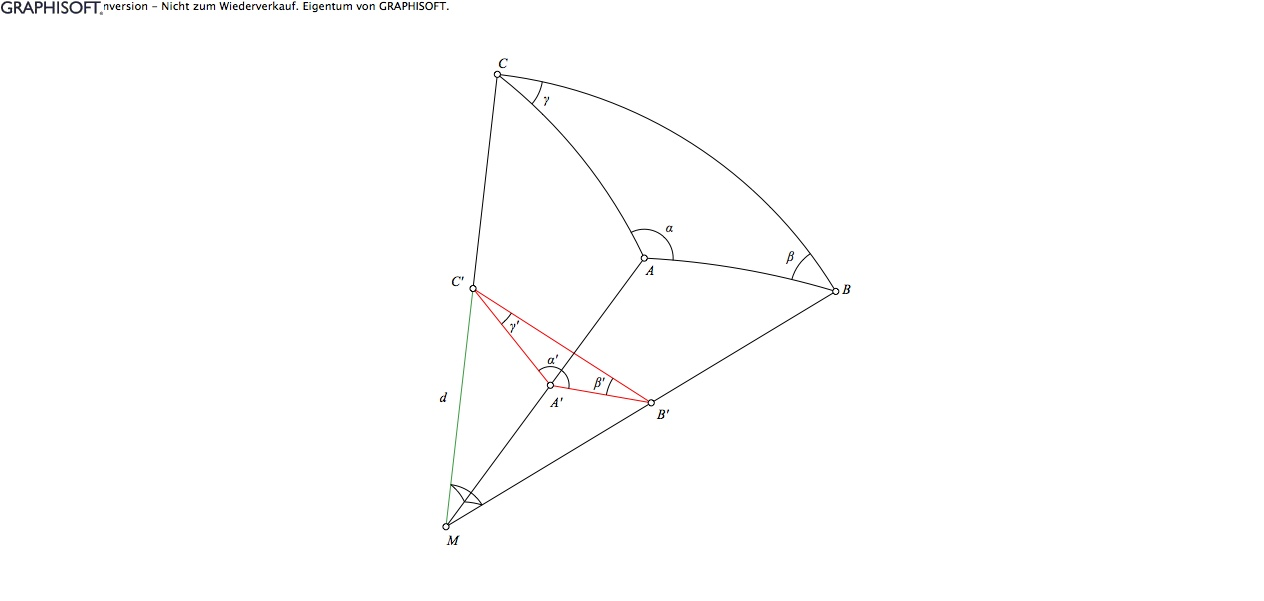
\includegraphics[width=0.5\textwidth]{kugel/1Seintenkosinus.jpg}
    \captionof{figure}{Bild Seitenkosinus}
\end{center}

Dabei lassen sich die Strecken nach den uns bekannten Regeln der Trigonometrie beschreiben:
\begin{align*}
\overline{C'A'} = d\cdot {tan(b)} \quad \quad \quad \quad \quad \quad 
\overline{MA'} = \frac{ d }{cos(b)} \\
\overline{C'B'} = d\cdot {tan(a)} \quad \quad \quad \quad \quad \quad 
\overline{MB'} = \frac{ d }{cos(a)}
\end{align*} 


Durch anwenden des Kosinussatzes der Ebene auf das Dreieck $A’B’C’$ erhalten wir
\begin{align}
\overline{A'B'}^{ 2 } &= \overline{ C'B' }^{ 2 } + \overline{ C'A' }^{ 2 } - 2 \cdot \overline{C'B'} \cdot \overline{ C'A' } \cdot cos(\gamma) \nonumber \\ 
\Rightarrow \quad \quad
\triangle \overline{A'B'}^{ 2 } &= d^{ 2 } \cdot \left(\left(tan^{ 2 }(a) + tan^{ 2 }(b)\right) - 2\cdot tan(a) \cdot tan(b) \cdot cos(\gamma)\right) 
\label {V3} 
\end{align}

dies gilt ebenso für das Dreieck $MA’B’$
\begin{align*}
\overline{A'B'}^{2} &= \overline{MB'}^{2} + \overline{MA'}^{2} - 2\cdot \overline{MB'} \cdot \overline{MA'} \cdot cos(c) \\
\Rightarrow \quad \quad
\overline{A'B'}^{ 2 } &= \left(\frac{ d }{ cos(a) }  \right)^{ 2 } + \left(\frac{ d }{ cos(b)}  \right)^{ 2 } - 2 \cdot \frac{ d }{ cos(a)} \cdot \frac{ d }{ cos(b)} \cdot cos(c) 
\end{align*}

Durch berücksichtigen von $\frac{1}{\cos^{2}(x)}=\tan^{2}(x)+1$ und ausklammern von $d^2$ folgt
\begin{align}
\overline{ A'B'}^{ 2 } &= d^{ 2 } \cdot \left(\left(tan^{ 2 }(a) + tan^{ 2 }(b)\right) - 2 \cdot \frac{ 1 }{ cos(a)} \cdot \frac{ 1 }{ cos(b)} \cdot cos(c)\right) 
\nonumber \\
\Rightarrow \quad \quad
\overline{ A'B'}^{ 2 } &= d^{ 2 } \cdot \left(\left(tan^{ 2 }(a) + 1\right) + \left(tan^{ 2 }(b) + 1\right) - \left(2 \cdot \frac{cos(c)}{cos(a) \cdot cos(b)}\right)\right)
\label {V4}
\end{align}

Durch gleichsetzen der beiden Gleichungen \eqref{V3} und \eqref{V4} können wir die Ausdrücke $d^2$ und $\tan^2(a) + \tan^2(b)$ streichen und erhalten

\begin{align*}
2 \cdot tan(a) \cdot tan(b) \cdot cos(\gamma) &= -2+2 \cdot \frac{cos(c)}{cos(a) \cdot cos(b)}
\end{align*}

Durch Umformung unter Einhaltung der Regel $\tan(a)=\frac{\sin(a)}{\cos(a)}$ und der Multiplikation mit  $\frac{1}{2}$ ergibt sich
\begin{align*}
\frac{\sin(a)}{\cos(a)} \cdot \frac{\sin(b)}{\cos(b)} \cdot \cos(\gamma) &= -1 + \frac{\cos(c)}{\cos(a) \cdot \cos(b)}
\end{align*}

Durch Vereinfachung erhalten wir den Seitenkosinussatz der Seite $c$
\begin{align*}
\cos(a) \cdot \cos(b) + \sin(a) \cdot sin(b) \cdot \cos(\gamma) = \cos(c)
\end{align*}

Um die Sätze für die Seiten $a$ und $b$ zu erhalten vertauschen wir die Variablen zyklisch und erhalten den Seitenkosinussatz.

\begin{satz}[\textit{Im sphärischen Dreieck ist der Kosinus einer Seite gleich der Summe der Kosinusprodukte der beiden anderen Seiten und dem mit dem Kosinus des eingeschlossenen Winkels multiplizierten Sinusprodukt dieser Seiten}]
\label{skript:kugel:satz:Seitenkosinussatz}
\index{Seitenkosinussatz}
\end{satz}

\begin{align*}
{\cos a} &= {\cos b} \cdot {\cos c} + {\sin b} \cdot {\sin c} \cdot {\cos \alpha}\\
{\cos b} &= {\cos c} \cdot {\cos a} + {\sin c} \cdot {\sin a} \cdot {\cos \beta}\\
{\cos c} &= {\cos a} \cdot {\cos b} + {\sin a} \cdot {\sin b} \cdot {\cos \gamma}\\
\end{align*}

Mithilfe des Seitenkosinussatzes lässt sich eine Dreieckesseite durch den gegenüberliegenden Winkel und die beiden anderen Seiten berechnen.



\subsection{Winkelkosinussatz}

Wenden wir den sphärischen Seitenkosinussatz auf dem Polardreieck an, erhalten wir
\begin{align*}
{\cos a} &= {\cos b} \cdot {\cos c} + {\sin b} \cdot {\sin c} \cdot {\cos \alpha}
\end{align*}

\begin{center}
        \includegraphics[width=0.3\textwidth]{kugel/Beispielbild.jpg}
    \captionof{figure}{Bild Winkelkosinus/Polardreieck}
\end{center}

Durch die Beziehung zwischen dem Polardreieck und dem sphärischen Dreieck, lässt sich der Seitenkosinussatz folgendermassen umformen
\begin{align*}
{\cos (\pi-\alpha)} &= {\cos (\pi-\beta)} \cdot {\cos (\pi-\gamma)} + {\sin(\pi-\beta)} \cdot {\sin(\pi-\gamma)} \cdot {\cos (\pi-a)}
\end{align*}

Durch die Quadrantenbeziehung der trigonometrischen Funktionen im Einheitskreis folgt

\begin{align*}
\sin (\pi-\alpha) &= \sin \alpha\\
\cos (\pi-\alpha) &= - \cos \alpha\\
\end{align*}

Es ergibt sich

\begin{align*}
{-\cos \alpha} &= {-\cos \beta} \cdot {-\cos \gamma} + {\sin \beta} \cdot {\sin \gamma} \cdot {-\cos a}
\end{align*}

Durch vertauschen der Vorzeichen erhalten wir den Winkelkosinussatz

\begin{satz}\textit{Im sphärischen Dreieck ist der Kosinus eines Winkels gleich der Summe aus dem negativen Produkt der Kosinus der beiden anderen Winkel und dem mit dem Kosinus der gegenüberliegenden Seite multiplizierten Sinusprodukt der beiden anderen Winkel.}
\label{skript:kugel:satz:Winkelkosinussatz}
\index{Winkelkosinussatz}
\end{satz}

\begin{align*}
{\cos \alpha} &= {-\cos \beta} \cdot {\cos \gamma} + {\sin \beta} \cdot {\sin \gamma} \cdot {\cos a}\\
{\cos \beta} &= {-\cos \gamma} \cdot {\cos \alpha} + {\sin \gamma} \cdot {\sin \alpha} \cdot {\cos b}\\
{\cos \gamma} &= {-\cos \alpha} \cdot {\cos \beta} + {\sin \alpha} \cdot {\sin \beta} \cdot {\cos c}\\
\end{align*}

Auf der Kugel können wir demnach zwei Kosinussätze anwenden und nicht nur einen wie in der Ebene. Den Seitenkosinussatz verwenden wir wenn mindestens 2 Seiten und 1 Winkel bekannt sind. Der Winkelkosinussatz lässt sich anwenden wenn mindestens 2 Winkel und 1 Seite bekannt ist. Mit beiden Sätzen können wir alle Unbekannten auf der Kugel herausfinden.



\section{Dualität auf der Kugel}

Durch die Herleitung des Winkelkosinussatzes haben wir zugleich die Dualität der Kugel bewiesen.

\begin{satz}\textit{Die sphärische Geometrie ist eine projektive Geometrie. In der projektiven Geometrie lassen sich alle Sätze dualisieren, das heisst, die Begriffe Punkt und Geraden werden vertauscht; demzufolge auch Längen und Winkeln}
\label{skript:kugel:satz:Dualitaet}
\index{Dualitaet}
\end{satz}

\begin{center}
        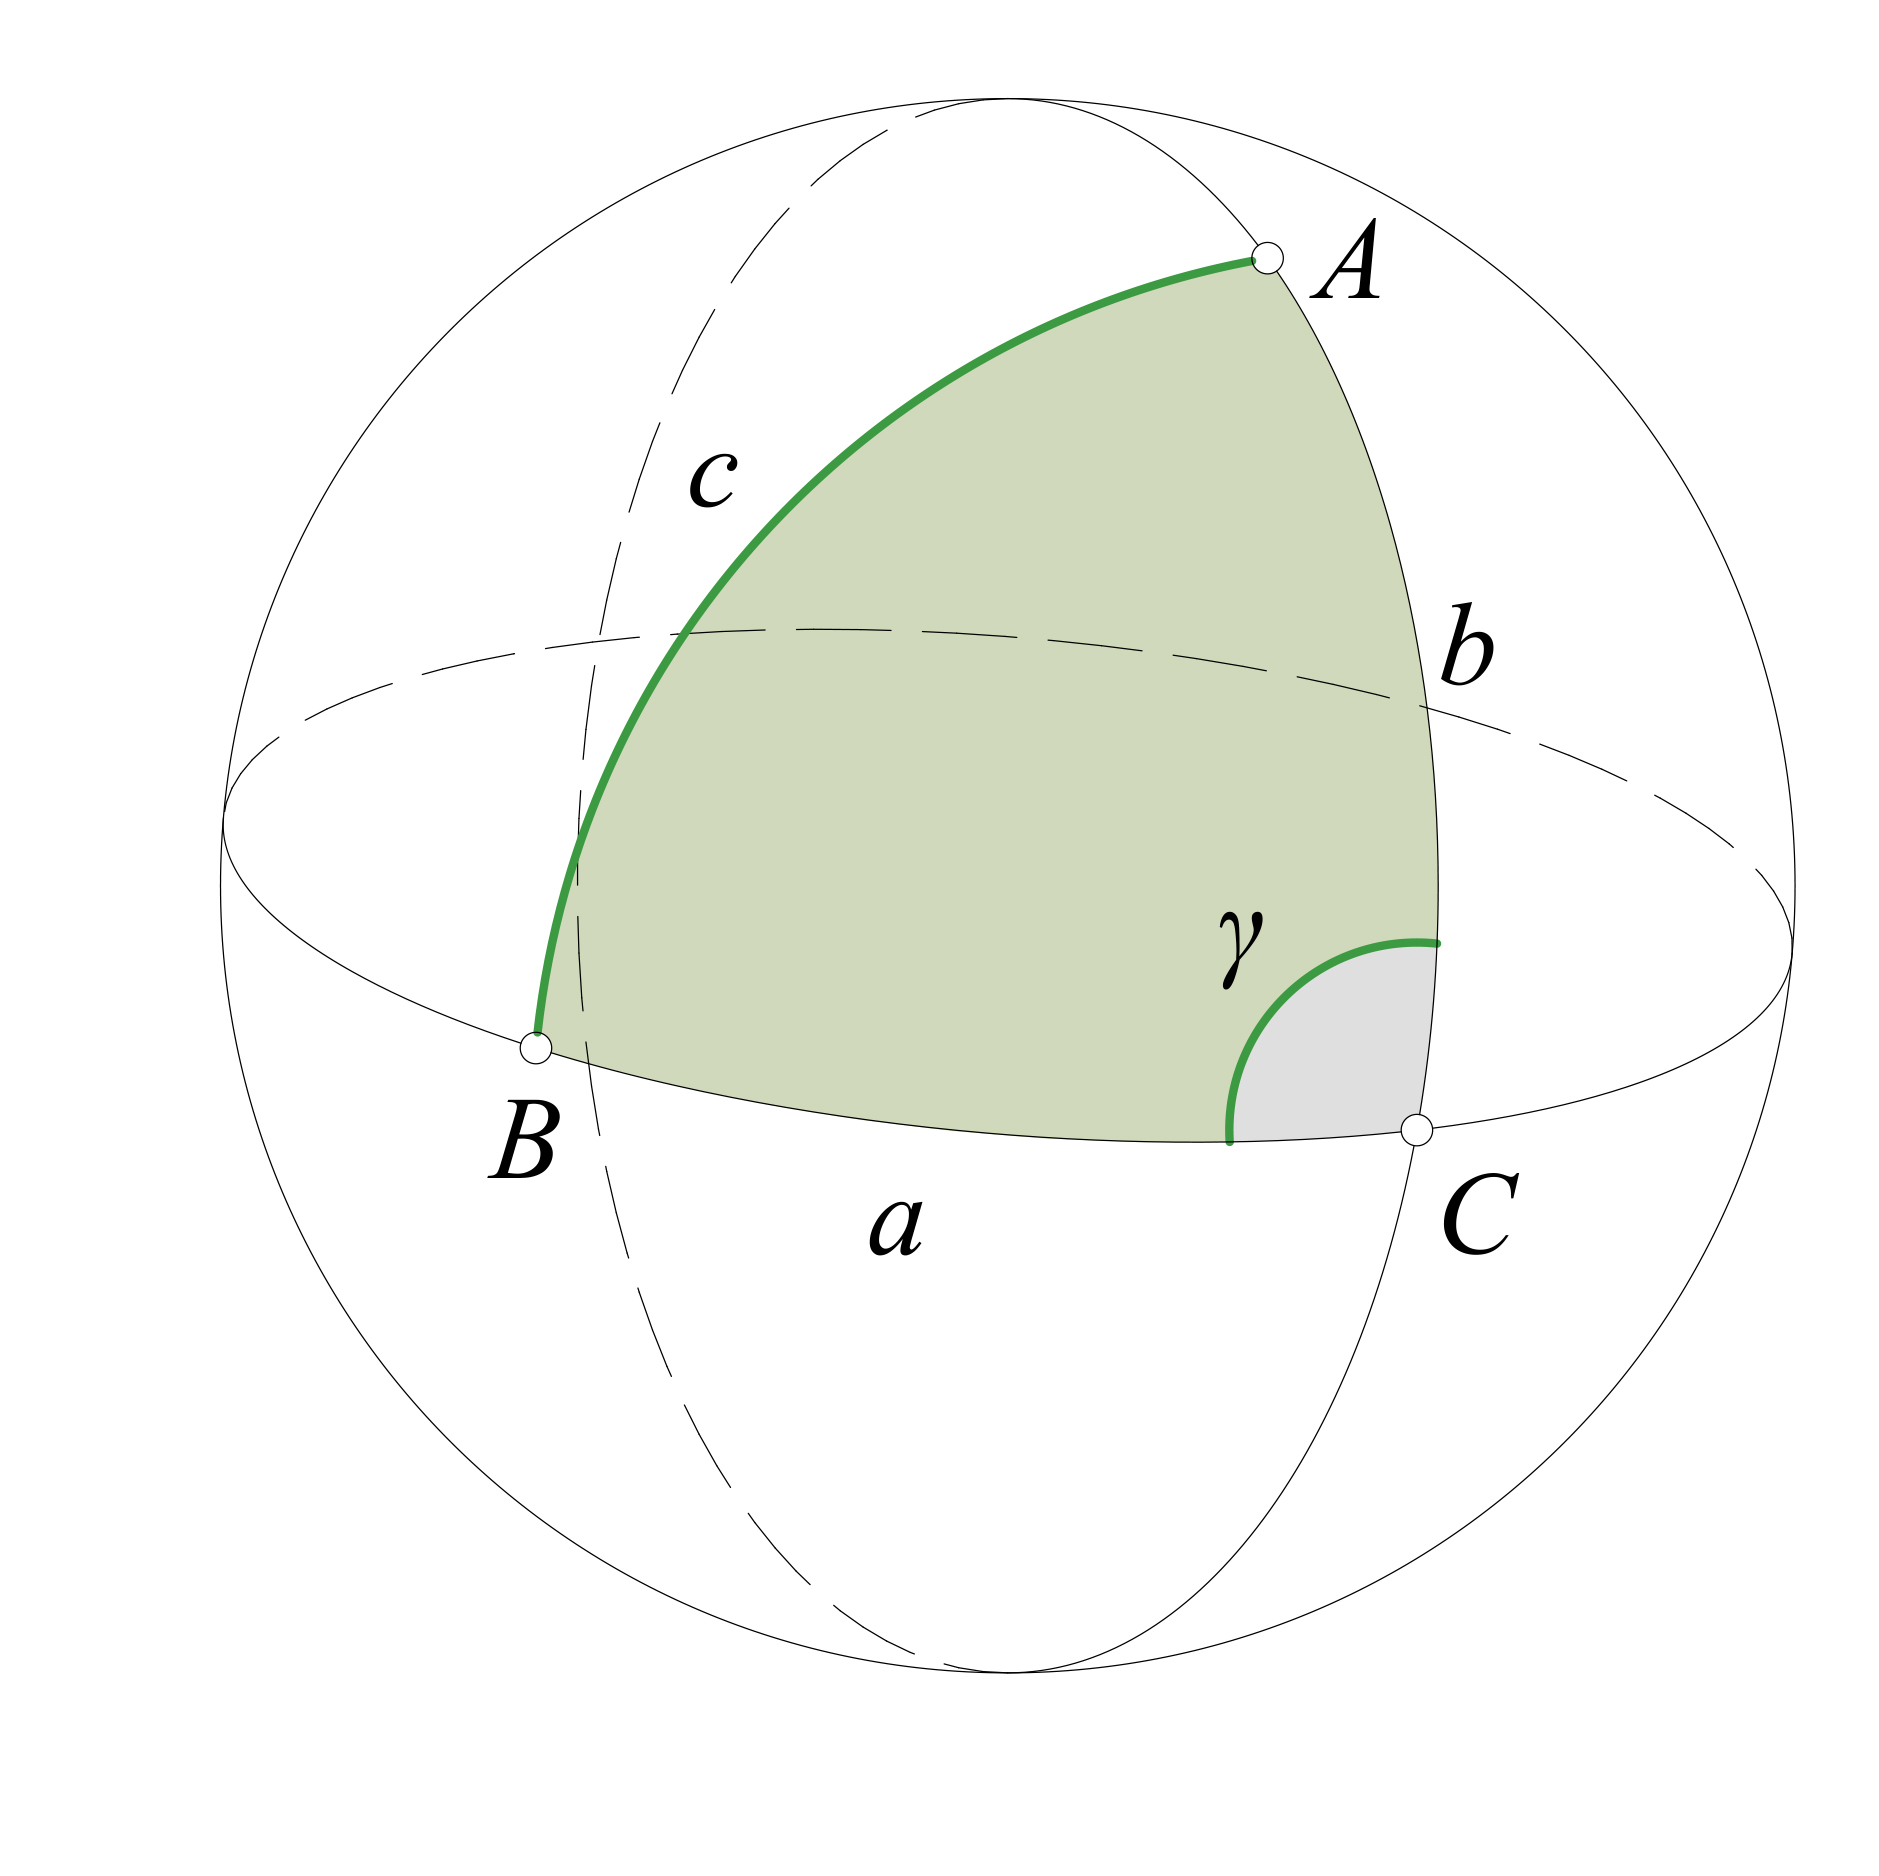
\includegraphics[width=0.4\textwidth]{kugel/_Dualitat.jpg}
    \captionof{figure}{Bild Dualität}
\end{center}

Nimmt man nun den Punkt $A$ welcher auf der Geraden $b$ liegt, so verläuft die Duale Gerade $a$ durch den zur Geraden $b$ dualen Punkt $B$. 
Aber nicht nur die Beziehungen zwischen Punkten und Längen bleiben erhalten. Auch die Winkel und Längen gehen ineinander über, wie im Beweis des Winkelkosinussatzes.
Der Winkel $\gamma$ zwischen den beiden Seiten $a$ und $b$ entspricht auf der Einheitskugel dem Abstand zwischen den zu der Geraden dualen Punkten $A$ und $B$.



\section{Navigation auf See}
Das besondere an Seekarten ist die Inhaltliche Ausrichtung. Anders wie Landkarten muss sie Informationen enthalten welche für den Kapitän und seine Besatzung von grosser Bedeutung sind. Vor allem in Küstennähe ist das navigieren eines Schiffes besonders gefährlich. So enthalten Seekarten etwas über die Wassertiefen, Bodenbeschaffenheiten, Gezeiten, Küstenlinien, Landzungen und Windrichtungen.
Der Hauptunterschied dabei ist, das auf der Landkarte feste Positionen definiert und aufgezeigt werden, das einzige was sich bewegt ist der Reisende selbst. Bei der Seekarte ist das anders, es werden veränderliche Einwirkungen der Natur festgehalten und die Schiffe auf See bewegen sich.

Dieser kleine Unterschied zeigt die Notwendigkeit auf, die Position und den Kurs seines Schiffes auf See immer ermitteln zu können.


\subsection{Geographische Koordinaten}
Bereits der griechische Astronom Claudius Ptolemäus verwendete in seiner Geographike Hyphegesis ein Gradnetz aus Längen- und Breitengraden. Dabei war sein Null-Meredian der bis ins 19. Jahrhundert verwendete Ferro-Meredian. Erst nach der Wiederentdeckung anfangs 15. Jahrhundert und der Übersetzung in die Lateinische Sprache setzte sich die Geographike Hyphegesis und damit das Ptolemäische Gradsystem durch. //
Mit dem Vertrag von Tordesillas von 1494 gewann das Gradnetz an politischer Bedeutung und bürgerlichte sich ein.
Im Jahr 1884 wurde der Nullmeredian Ferro-Meredian durch den noch heute gültigen Greenwich Meredian welcher in Grossbritannien seit 1738 in gebrauch war ersetzt.

Zur geografischen Ortsbestimmung und damit der Festlegung seines eigenen Standortes auf einer Karte sind Längen- und Breitengrad nötig. \\
Die Koordinaten werden traditionell im Sexagesimalsystem angegeben und setzen sich aus folgenden Komponenten zusammen:
\[
\begin{aligned}
&\text{Grad } (^{\circ})
&
&\text{\bigg \vert}
&
&\text{Bogenminuten } (`)
&
&\text{\bigg \vert}
&
&\text{Bogensekunden } (``)
\end{aligned}
\]

Die Erdoberfläche wurde in je 360 Breiten- und Längengrade eingeteilt. Die Breitengrade haben zueinander einen Abstand von 111.31 km, dies entspricht auch dem Abstand der Längengrade am Äquator, welcher mit Zunehmender Nähe zu den Polen ab nimmt.
\[
\begin{aligned}
&1^{\circ}
&
&\text{\bigg \vert}
&
&4 \text{ Minuten}
&
&\text{\bigg \vert}
&
&111.31\text{ km}
\end{aligned}
\]

Eine ganze Erdumdrehung sind $360 ^{\circ}$ was 1440 Minuten entspricht, dabei erhält man genau den Erdumfang am Äquator:
\begin{align*} 40’074 \text{ km.}\end{align*}

Nach einer vollen Umdrehung der Erde stellt sie sich wider in ihrer Ursprungsposition ein und ein neuer Tag beginnt. Dies Zeit das die Koordinaten in direkten Zusammenhang mit der Zeit stehen, diese Erkenntnis wird später für die Navigation auf See von grosser Bedeutung.


\subsection{Erdachsenneigung}
Die Erdachse oder auch Rotationsachse genannt ist um ca. $23.5^{\circ}$ geneigt.
Dadurch lassen sich Phänomene wie die vier Jahreszeiten oder die verschiedenen längen der Tage beobachten.
Für die nautische Navigation hat die Erdneigung eine grosse Bedeutung, da je nach Neigung andere Sterne zu beobachten sind, auch ist die Sonne an einem anderen Ort am Himmel zu finden.

\begin{center}
        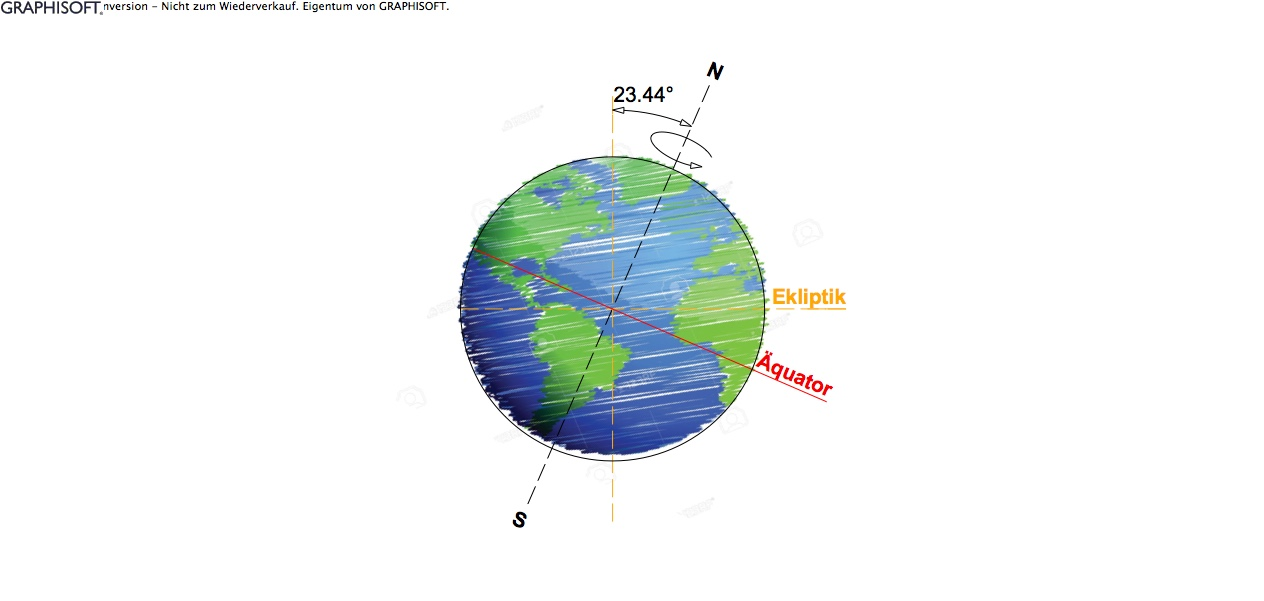
\includegraphics[width=0.5\textwidth]{kugel/1Ekliptik.jpg}
    \captionof{figure}{Bild Erdneigung}
\end{center}


XXXX

Der Himmelsäquator ist die Linie, die orthogonal zur Sonne verläuft.
Die Ekliptik-Linie ist die Linie, die orthogonal zur Erdachse verläuft.
Der Schnittpunkt dieser Kreise wird als Frühlings- / Herbstpunkt bezeichnet und ist jeweils am 21. März / 21. Oktober des Jahres.
Der Frühlingspunkt $\Upsilon$ wird oft als Gestirnspunkt im nautischen Dreieck verwendet, genaueres wird im Kapitel zum nautischen Dreieck erklärt.


XXXX

\subsection{Zeitzonen der Erde} \label{Zeitzonen} 
Wenn man nun die verschiedenen Zeitzonen der Erde betrachtet, macht die Verschiebung von jeweils genau einer Stunde durchaus Sinn, es lässt sich auf die Längengrade schliessen.
Zwischen den verschiedenen Zeitzonen liegen 15 Längengrade:
\begin{align*}
\text{15 Längengrade à 4 Minuten = 60 Minuten Zeitverschiebung = ca. 1665 km}
\end{align*}

Dabei ist die Zeitzone in welcher Mitte sich der Greenwich Meredian befindet die \textit{Greenwich Mean Time (GMT)} welche bis 1928 als Weltzeit galt. Im Jahr 1972 wurde diese umbenannt in die \textit{Coordinated Universal Time (UTC)} und wir von da an als Weltzeit $\pm$ 0.00 verwendet, der Meredian blieb der selbe.


\section{Der Breitengrad}
Die Breitengrade bilden die bereits genannten Kleinkreise auf der Kugeloberfläche. Sie verlaufen in einem Abstand von etwa 111 km parallel zum Äquator. Dabei stellt dieser genau die Mitte zwischen Nord- und Südpol dar und teilt die Erdkugel in zwei gleich grosse Hälften. Dabei bildet der Äquator den natürlichen Nullpunkt der Breitengrade. Um zu wissen auf welcher Halbkugel man sich befindet, spricht man von nördlicher und südlicher breite oder gibt die Werte für Nord Positiv und für Süd Negativ an.e.

\begin{center}
        \includegraphics[width=0.3\textwidth]{kugel/Beispielbild.jpg}
    \captionof{figure}{BILD SKIZZE DER GEOGRAFISCHEN BREITE ERDKUGEL}
\end{center}


\subsection{Geografische Breite $\phi$}
\begin{definition}
Die geografische Breite eines Standortes ist nichts anderes, als der Winkel am Erdmittelpunkt zwischen der Ebene des Äquators und der Geraden zum Standpunkt auf der Erdoberfläche.
\end{definition}

\begin{center}
        \includegraphics[width=0.3\textwidth]{kugel/Beispielbild.jpg}
    \captionof{figure}{Bild}
\end{center}


\subsection{Navigation mit den Breitengraden}  \label{BreitengradM}
Da der Breitengrad bereits sehr früh ziemlich präzise bestimmt werden konnte, nutzten bereits die Seefahrer um Christoph Kolumbus den Breitengrad zur Navigation ihrer Flotten.
Den dieser lässt sich ziemlich einfach aus dem höchsten Sonnenstand oder einem Fixstern bestimmen. Dabei wird mit einem Jakobsstab\footnote{%
Der Jakobsstab ist ein früheres astronomisches Instrument zur Winkelmessung und wurde vor allem in der Seefahrt verwendet. Er ist in der Nautik der Vorläufer des Sextanten.} (später Sextant\footnote{%
Der Sextant ist ein nautisches Messinstrument zur Winkelmessung von Horizont und Fixstern (Gestirn)}) der Winkel zwischen dem Horizont und dem höchsten Sonnenstand oder einem Fixstern gemessen. Der Winkel welchen man erhält, zieht man von 90° ab und erhält somit die geografische Breite. \\

\begin{center}
        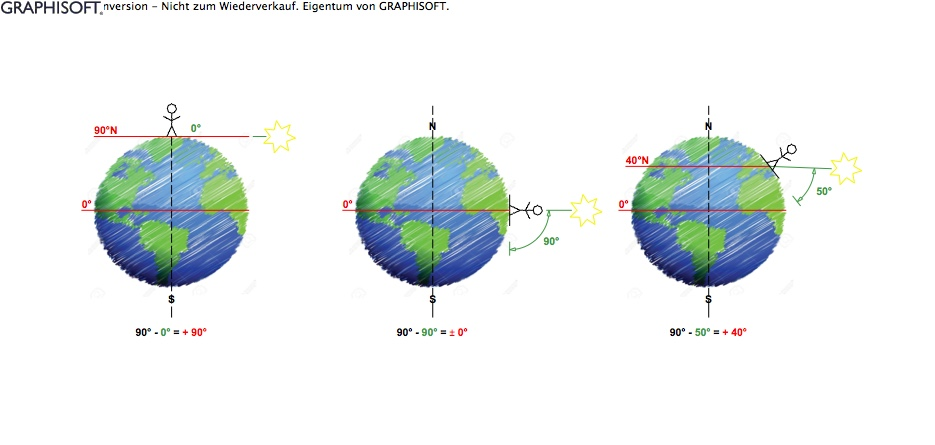
\includegraphics[width=1\textwidth]{kugel/1Breitengrad.jpg}
    \captionof{figure}{Bild}
\end{center}

Wenn man sich auf der Nordhalbkugel befindet, ist der Polarstern ein sehr guter Fixstern. Befindet sich ein Schiff nun sehr nahe am Nordpol, steht dieser nahezu senkrecht am Himmelszelt bei $90^{\circ}$. Würde es aber nahe dem Äquator stehen, erscheint dieser am Horizont bei $0^{\circ}$ und wäre je nach dem nicht mehr zu sehen.


\subsection{Korrekturbeiwert}
Da Breitengrade Kleinkreise sind, haben auch diese nicht immer den selben Radius. Daher segelt man am Äquator viel länger dem Breitengrad entlang um zum nächsten Längengrad zu kommen als in der nähe des Nord- oder Südpols.

\[
\begin{aligned}
&\text{1}^{\circ}
&
&\text{\bigg \vert}
&
&\text{4 Minuten}
&
&\text{\bigg \vert}
&
&\text{111.13 km}
\\
\\
&\text{0.25}^{\circ}
&
&\text{\bigg \vert}
&
&\text{1 Minute}
&
&\text{\bigg \vert}
&
&\text{27.78 km}
\\
\\
&\text{0.004166}^{\circ}
&
&\text{\bigg \vert}
&
&\text{1 Sekunde}
&
&\text{\bigg \vert}
&
&\text{463m}
\end{aligned}
\]

Um die verminderte Strecke zu erhalten, müssen wir den Cosinus des gemessenen Breitengrades berechnen und diesen mit der Abweichung auf dem Äquator von 1 Sekunde multiplizieren.

\begin{center}
        \includegraphics[width=0.3\textwidth]{kugel/Beispielbild.jpg}
    \captionof{figure}{Bild}
\end{center}

\[
\begin{aligned}
&\cos 90^\circ \cdot 463\text{m} = 463\text{m}
&
&\text{\bigg \vert}
&
&\cos 50^\circ \cdot 463\text{m} = 297.61\text{m}
&
&\text{\bigg \vert}
&
&\cos 0^\circ \cdot 463\text{m} = 0\text{m}
\end{aligned}
\]

Dies zeigt, je näher man den Polen ist, desto weniger weit muss man Segeln um den nächsten Längengrad zu erreichen.



\section{Der Längengrad}
Die Längengrade bilden die bereits genannten Grosskreise auf der Kugeloberfläche.
Sie schneiden den Äquator im rechten Winkel, haben dort einen Abstand von etwa 111 km zueinander. Sie verbinden die beiden Pole Nord und Süd miteinander. Anders als bei der geografischen Breite, ist in der Natur kein Längengrad gegeben welcher den Nullpunkt darstellt.

\begin{center}
        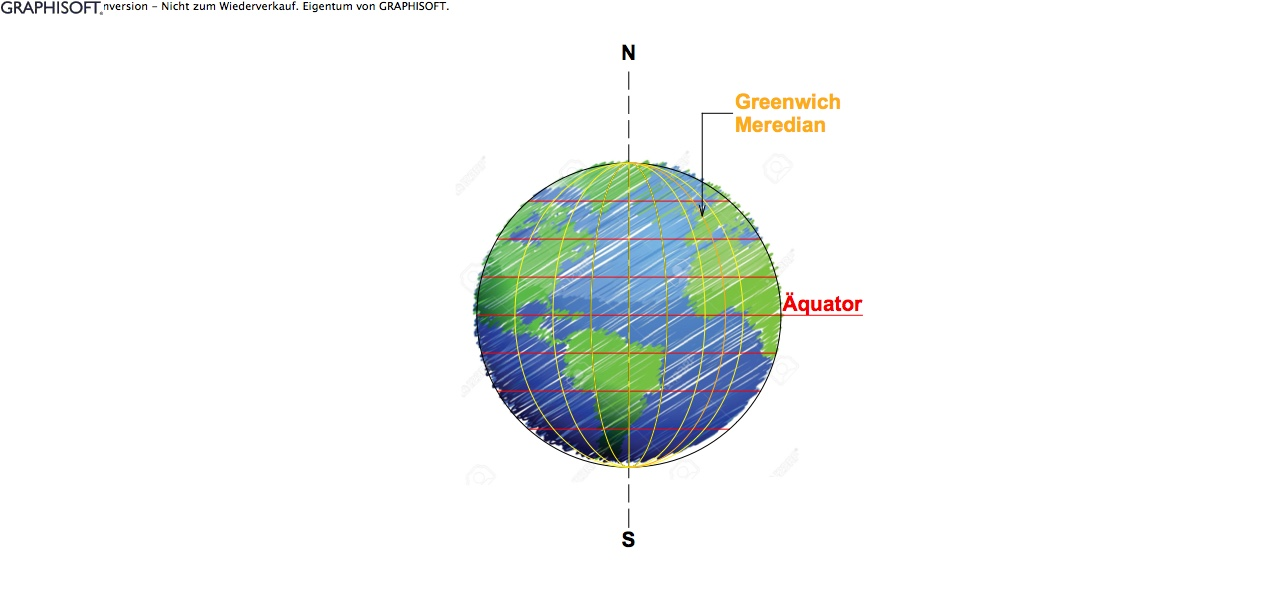
\includegraphics[width=0.5\textwidth]{kugel/1Langengrad.jpg}
    \captionof{figure}{Bild}
\end{center}


\subsection{Geografische Länge $\lambda$}
\begin{definition}
Die geografische Länge ist der Winkel an der Erdachse zum Nullmeridian.
\end{definition}

\begin{center}
        \includegraphics[width=0.3\textwidth]{kugel/Beispielbild.jpg}
    \captionof{figure}{Bild}
\end{center}

\subsection{Navigation mit den Längengraden}
Die geografische Länge lässt sich nicht so einfach bestimmen wie deren Breite.
Für die Berechnung auf See benötigt man eine Referenzzeit eines Ortes mit bekannter Länge.
In der Zeit der Entdecker gab es noch keine mechanischen Uhren. Die Sonnenuhr war zudem ungeeignet, da diese nur die Uhrzeit am Standort mass und nicht die am Referenzort selbst. Die erste Pendeluhr wurde Mitte des 17. Jahrhunderts erfunden, was in der Schifffahrt aber auch nicht die Lösung brachte.\\
Pendeluhren auf einem Schiff sind ungeeignet, da das Pendel mit dem Wellengang aus dem Takt gebracht wird und somit die Uhr falsch geht.
Zu ungenau und gegen äussere Erschütterungen sehr empfindlich waren später die federgetriebene Uhren und die Unruh. Dazukamen die verschiedenen Klimazonen welche ein Schiff zu durchqueren hatten. Das Metall zog sich viel zu fest zusammen oder dehnte sich aus, was dazu führte das die Uhr unregelmässig lief.

Das sogenannte „Längenproblem“ stellte nicht nur in der Navigation auf See ein Problem dar, auch die Wirtschaft hatte darunter zu leiden. Die Schiffe mussten bis zur gewünschten geografischen Breite navigieren und segelten dann den Breitengrad entlang um auch wirklich auf der gewünschten Position anzukommen. Dabei waren die Schiffe oft Wochenlang unterwegs und segelten die „Breiten ab“ um an die gewünschte Positionen zu kommen. Dies führte zu erheblichen Zeitverlusten und viel längeren Reisezeiten.



\section{The Board of Longitude - Das Längenproblem}
Das Längenproblem beschäftigte alle grossen Seefahrernationen Europas. Die fehlenden Längengrade bei der Navigation führten zu vielen Schiffsunglücken. Nicht selten kam es vor, das sich auf den untergegangenen Schiffen Schätze in der Höhe von halben britischen Staatshaushalten befanden. Der Verlust solcher Schiffe war enorm.\\
Bereits um 1600 hatte der König von Spanien ein Preisgeld ausgeschrieben für denjenigen welcher eine Lösung für das Problem präsentieren konnte. Leider ohne Erfolg. \\
Nach einem tragischen Unglück im Jahr 1707, beidem der siegreiche Admiral Sir Cloudesley und seine 1’450 Mann sein Leben liessen, indem sie auf die Scilly-Inseln kurz vor Land’s End aufliefen und dabei die 21 Schiffe sanken, rückte das Problem wieder in den Vordergrund.
Sieben Jahre später, und mithilfe einer Petition von William Whiston und Humphry Ditton welche von Sir Isaac Newton und Edmond Halley untermauert wurde, reagierte das britische Parlament.
Es schrieb folgende Preisgelder für eine praktisch, brauchbare Lösung aus:
\[
\begin{aligned}
&\text{20’000£}
&
&\text{\big \vert}
&
&\text{Für eine Abweichung von max.} \frac{1}{2}^{\circ} \text{(etwa 55.5 km am Äquator)}
\\
\\
&\text{15’000£}
&
&\text{\big \vert}
&
&\text{Für eine Abweichung von max.} \frac{2}{3}^{\circ} \text{(etwa 74 km am Äquator)}
\\
\\
&\text{10’000£}
&
&\text{\big \vert}
&
&\text{Für eine Abweichung von max.} 1 ^{\circ} \text{(etwa 111 km am Äquator)}
\end{aligned}
\]
Eine Abweichung von 111km am Äquator entspricht 60 Seemeilen.
Auf der Höhe des Ärmelkanals und damit nahe Londons, beträgt die Abweichung nur $1 ^{\circ}$ noch 74km und somit 40 Seemeilen.//
Das Preisgeld entsprach einer enorm hohen Summe für diese Zeit. Der Kaufpreis für ein mittleres Schiff welches zur See fahren konnte lag bei etwa 1’500-2’500£, ein einzelner Arbeiter lebte mit 10£ im Jahr.
Würde man dieses Problem heute mit einer Abweichung von maximal einem halben Grad lösen, erhielte man 2’840’000£ was etwa einem Wert von 3’600’000 Schweizer Franken entspräche. 

Damit die Lösungsvorschläge kontrolliert und verwaltet werden konnten, wurde die Board of Longitude (Längenkommission) gegründet. Ihr gehörten die bedeutendsten Astronomen und Mathematiker dieser Zeit an, aber auch berühmte Persönlichkeiten aus Grossbritannien wie der Präsident der Royal Society und damit niemand anderen als Sir Issac Newton.


\subsection{John Harrison}
Harrison brachte sich das Handwerk des Uhrmachers selbst bei. Im Alter von 20 Jahren im Jahr 1713 konstruierte er seine erste Pendeluhr. In den weiteren Jahren folgten noch weitere Pendeluhren und Standuhren. Durch die Einführung der Grasshopper-Hemmung und des Rostpendels, erreichten die Uhren eine enorme Genauigkeit für die damalige Zeit. Die Abweichung pro Monat betrug dabei nur etwa eine Sekunde. \\
Erst 13 Jahre nach der Ausschreibung für die Lösung des Längenproblems tüftelte er an einer Konstruktion für eine Schiffsuhr und setzte sich mit dem Längenproblem auseinander.
Namhafte Astronomen in ganz Europa suchten nach astronomischen Lösungen für das Problem, Harrison jedoch setzte auf genaue Uhren und war somit unabhängig davon ob man den Mond sah oder nicht.\\
1728 folgte sein erstes Konzept für eine schiffstaugliche Uhr, 1735 präsentierte er sein erstes Modell die H1.
Die Testfahrt mit der H1 an Board von London nach Lissabon und zurück, hielt die vorgeschriebene Genauigkeit ein und übertraf diese sogar. Jedoch hatte die Reisedauer nicht den vorgeschriebenen Bedingungen entsprochen.\\
Das Hauptproblem war jedoch, das Harrison als nichtstudierter Laie einem gelehrten Gremium dem Board of Longitude gegenüber stand. Dies verzögerte seine Annahme um Jahrzehnte. Der Krieg zwischen Spanien und Grossbritannien spielte ihm ebenfalls nicht in die Karten. Seine weiteren Uhren die H2 und H3 wurden nie getestet, da man nicht wollte das der Feind eine dieser Uhren in die Hände bekam.

\begin{center}
        \includegraphics[width=0.3\textwidth]{kugel/JohnHarrison.jpg}
    \captionof{figure}{Bild John Harrison}
\end{center}

\begin{center}
        \includegraphics[width=0.2\textwidth]{kugel/HarrisonH4.jpg}
    \captionof{figure}{Bild Harrison's H4}
\end{center}

Mit einem Durchmesser von 13cm und 1.45kg folgte im Jahr 1753 endlich der Durchbruch.
Die Taschenuhr H4 stellte alle anderen Uhren in den Schatten. Auf einer 81-tägigen Fahr nach Jamaika zeigte sie eine Abweichung von nur 5 Sekunden.
Das Gremium entschied erneut gegen Harrison und beauftragte ihn seine Uhr vor ihren Augen zu zerlegen, zu erklären und Konstruktionszeichnungen anzufertigen.
Nachdem Harrison vom britischen Parlament ein Preisgeld in der Höhe von 10’000£ erhalten hatte um mit diesem Geld eine Kopie anzufertigen, um den Beweis zu liefern das seine Uhr nicht nur zufällig so genau lief.\\
Der bekannte Londoner Uhrmacher Larcum Kendall fertigte danach eine Kopie der H4 an und zeigte somit das die Uhr den Anforderungen entsprach.\\
Das Geld blieb für Harrison aber weiterhin aus. Erst nachdem der britische König Georg III dem Parlament angedroht hatte persönlich zu erscheinen und Harrison das Geld zuzusprechen, schrieben dieses ihm 3 Jahre vor seinem Ableben weitere 8750£ zu.\\
8 Monate vor seinem Tod und der Rückkehr der K1 (Kopie der H4) ging die Vision Harrisons in Erfüllung, es war nun definitiv bewiesen das seine Uhr auf dem offenen Meer zur Bestimmung des Längengrades taugte. James Cook der berühmte britische Seefahrer und Entdecker welcher die Uhr K1 auf See mitnehmen und testen durfte, nannte die Uhr liebevoll seinen \textit{nie versagenden Führer}.
Auf der Grundlage Harrisons H4 wurden die Schiffschronometer noch lange Zeit gebaut.



\subsection{Tobias Mayer}
Etwa zur gleichen Zeit wie John Harrison entwickelte Tobias Mayer\footnote{%
Tobias Mayer (1723-1762) studierte nie an einer Universität und war trotzdem ein annerkannter Wissenschaftler seiner Zeit in den Bereichen Astronomie, Geo- und Kartograf, Mathematiker und Physiker.}  ebenso eine Lösung für das Längenproblem. Obschon er nie an 


\begin{center}
        \includegraphics[width=0.3\textwidth]{kugel/TobiasMayer.jpg}
    \captionof{figure}{Bild}
\end{center}

Seine Mondkarten galten ein halbes Jahrhundertlang als unübertroffen. Der Ruhm galt aber hauptsächlich seinen Mondkarten welche er im Jahr 1755 in einer erweiterten Version dem britischen Parlament vorlegte.\\
Mit ihnen konnte man die Geografische Länge bis auf 5 Bogensekunden genau bestimmen. Dies entsprach am Äquator $0.5 ^{\circ}$, was wiederum eine Genauigkeit von 55.565km entsprach.\\
Eine Lösung für das Längenproblem war gefunden. Die Publikation seiner Mondtafeln fand 1767 unter dem Titel \textit{Theoria lunae juxta systema Newtonianum} in London statt, 5 Jahre nach Mayers Tod. 
Seine Witwe schickte die publizierten Mondkarten über die Universität Göttingen nach Grossbritannien. Sie erhielt von der britischen Regierung eine Prämie in der Höhe von £ 3’000.-.

Im Jahr 1935 wurde ein Krater auf der westlichen Mondvorderseite nach dem deutschen Astronomen benannt, er trägt fortan den Namen T.Mayer.

\begin{center}
        \includegraphics[width=0.3\textwidth]{kugel/Mondkarte.jpg}
    \captionof{figure}{Mondkarte}
\end{center}


\begin{figure} 
    \subfigure[Bezeichnung der linken Grafik]{\includegraphics[width=0.3\textwidth]{kugel/Mondkarte.jpg}}
    \subfigure[Bezeichnung der rechten Grafik]{\includegraphics[width=0.3\textwidth]{kugel/Mondkarte.jpg}} 
\caption{Titel unterm gesamten Bild} 
\end{figure} 


XXXXXXX


\section{Nautisches Dreieck (Astronomisches Dreieck)}
Um seine Koordinaten bestimmen zu können, genauer gesagt um den Längengrad zu ermitteln ohne moderne GPS-Geräte, ziehen wir ein altbewährtes Hilfsmittel aus der Seefahrt zur Hilfe - Das Nautische Dreieck. \\
Es dient zur Positionsbestimmung auf dem offenen Meer oder anderen Gebieten in denen keine Orientierungspunkte wie Landzungen oder Gebirgsketten zu Hilfe genommen werden können.

Das Nautische Dreieck an der Himmelskugel hat folgende Eckpunkte:
\begin{itemize}
\item Himmelsnordpol ($N$) - auch bekannt als Polarstern
\item Gestirn ($S$) - ein uns bekannter Stern, wir verwenden im Beispiel die Sonne
\item Zenit ($Z$) - der Himmelspunkt welcher sich senkrecht über uns befindet
\end{itemize}

Dieses Kugeldreieck wird das nautisches Dreieck genannt.

%SKIZZE NAUTISCHES DREIECK

\subsection{Berechnung der Dreiecksseiten}

\begin{align*}
\overline{ZS} = 90^{\circ} - h \quad \quad \quad \quad \quad \quad 
\overline{NZ} = 90^{\circ} - \phi \\
\overline{NS} = 90^{\circ} - \delta \quad \quad \quad \quad \quad \quad 
\tau = t - e_\delta - \lambda 
\end{align*}
 

\subsection{Bestimmung des Längengrades} \label{BestimmungL} 
Zur Bestimmung des Längengrades verwenden wir den Seitenkosinussatz:
\begin{align*}
\cos(c) = \cos(a)\cos(b) + \sin(a)\sin(b)\cos(\gamma)
\end{align*}

Auf unsere Seiten angewendet können wir einsetzen

\begin{align*}
\cos(\overline{ZS}) &= \cos(\overline{NZ}) \cos(\overline{NS}) + \sin(\overline{NZ}) \sin(\overline{NS}) \cos(\tau) \\
\Rightarrow \quad \quad
\cos(90^{\circ} - h) &= \cos(90^{\circ} - \phi) \cos(90^{\circ} - \delta) + \sin(90^{\circ} - \phi)\sin(90^{\circ} - \delta) \cos(\tau)
\end{align*}

Nach dem uns unbekannten Winkel $\tau$ aufgelöst ergibt die Gleichung
\begin{align*}
\tau = \arccos 
\frac{ \cos(90^{\circ} - \phi) \cos(90^{\circ} - \delta) - \cos(90^{\circ} - h)} {\sin(90^{\circ} - \phi)\sin(90^{\circ} - \delta)}
\end{align*}

Der Winkel $\tau$ setzt sich aus folgenden Komponenten zusammen
\begin{align*}
\cos (\tau) = \cos (t - e_\delta - \lambda) 
\end{align*}

Dabei haben wir diese uns bekannten Grössen:
\begin{itemize}
\item Zeit ($t$) $\Rightarrow$ Uhr
\item Rektazension ($e_\delta$) $\Rightarrow$ Sternatlas, Almanach, App 
\end{itemize}
\\

Dabei ist die einzige Unbekannte der gesuchte Längengrad ($\lambda$), dieser lässt sich 
\begin{itemize}
\item Längengrad ($\lambda$) $\Rightarrow$ Der Längengrad unseres Standorts ist die einzige Unbekannte
\end{itemize}

\subsection{Sternzeit}


\subsection{Breitengrad bekannt? - Breite nicht bekannt!}
In den vorherigen Berechnungen sind wir immer davon ausgegangen, das uns die Breite bekannt ist. Dies ist in Wirklichkeit aber nicht so, denn auf dem offenen Meer hat man keinerlei Anhaltspunkte wo man sein könnte. \\
Im Kapitel~\ref{BreitengradM} \nameref{BreitengradM} haben wir aber gesehen, das sich dieser relativ einfach und ohne grossen Aufwand bestimmen lässt. Damit wir auf See eine verlässliche Messung erhalten, benötigen wir mindestens zwei Sterne. Mit diesen beiden Messungen kann man den Messfehler minimieren und den Standort relativ genau bestimmen.

Da wir zwei Sterne haben, benötigen wir auch zwei Gleichungen mit zwei Unbekannten
\begin{align*}
\cos(\overline{ZS_1}) &= \cos(\overline{NZ}) \cos(\overline{NS_1}) + \sin(\overline{NZ}) \sin(\overline{NS_1}) \cos(\tau_1) \\
\cos(\overline{ZS_2}) &= \cos(\overline{NZ}) \cos(\overline{NS_2}) + \sin(\overline{NZ}) \sin(\overline{NS_2}) \cos(\tau_2) \\
\\
\Rightarrow \quad \quad
\cos(90^{\circ} - h_1) &= \cos(90^{\circ} - \phi) \cos(90^{\circ} - \delta_1) + \sin(90^{\circ} - \phi)\sin(90^{\circ} - \delta_1) \cos(\tau_1) \\
\Rightarrow \quad \quad
\cos(90^{\circ} - h_2) &= \cos(90^{\circ} - \phi) \cos(90^{\circ} - \delta_2) + \sin(90^{\circ} - \phi)\sin(90^{\circ} - \delta_2) \cos(\tau_2)
\end{align*}

Diese Gleichungen lassen sich nur mit Hilfe eines Computers oder viel Geduld und Zeit lösen. Die Hilfe des Computers ist heutzutage kein Problem, jedoch gab es diesen zur Zeit der Entdecker und Seefahrer nicht. Da kommt die Geduld und Zeit ins Spiel, diese war auf einem Schiff auf offener See reichlich vorhanden.





\printbibliography[heading=subbibliography]
\end{refsection}



